\documentclass[12pt,a4paper,oneside,titlepage]{report}

%\textwidth=15cm
%\hoffset=-1 cm
\usepackage{ngerman}
\usepackage[latin1]{inputenc}
\usepackage{ae}
\usepackage{graphicx}
\usepackage{amsmath}
\usepackage{amsthm}
\usepackage{dsfont}
\usepackage{listings}
%\usepackage{amsfonts,textcomp}
%\usepackage{calc}

\usepackage{makeidx,showidx} \makeindex
\usepackage{multirow}
\usepackage{tabularx}
\usepackage{subfigure}
\usepackage{epic}
\usepackage{longtable}
\usepackage{rotating}
\usepackage{float}
\usepackage{fancyvrb}
%\usepackage{glossary}
%URL Farb und Link Anpassung
%\usepackage{fancyhdr}
\usepackage{color}
\usepackage{hyperref}
\usepackage{lscape}
\definecolor{black}{rgb}{0,0,0}
\definecolor{darkblue}{rgb}{0,0,0.5}
\hypersetup{colorlinks, linkcolor=black, urlcolor=darkblue, citecolor=black, pdftitle={Konzeption und Evaluation von Instruktionssatzerweiterungen zur Optical Flow Berechnung f�r einen ASIP}, pdfauthor={Kristian Wolpers}, pdfsubject={Bachelorarbeit, September 2010}}


\renewcommand{\arraystretch}{1.5}
\newcommand\textsubscript[1]{\ensuremath{{}_{\text{#1}}}}

\addtolength{\headheight}{0,3cm}
\addtolength{\headsep}{-0,3cm}
\setlength{\parindent}{0pt}
\setlength{\parskip}{12pt plus 6pt minus 3pt}
\setlength{\partopsep}{0pt}
\addtolength{\topmargin}{-0,6cm}
\addtolength{\oddsidemargin}{-0,6cm}
\addtolength{\textwidth}{2cm}
\addtolength{\textheight}{2cm}

\restylefloat{figure}
\IfFileExists{url.sty}{\usepackage{url}}

\usepackage{fancyhdr}
\pagestyle{fancy}


\renewcommand{\headrulewidth}{0.4pt}
\renewcommand{\sectionmark}[1]{\markright{ Kapitel  \thesection\ \it #1}}
\renewcommand{\chaptermark}[1]{\markright{ Kapitel  \thechapter\ \it #1}}

\lhead{\nouppercase{\rightmark}}
\rhead{\thepage}
\cfoot{}

% Damit auch die Titelseiten fancy sind!
\makeatletter
\let\ps@plain=\ps@empty
\makeatother

%Fourier-Korrespondenz link  *-o

\newcommand{\ftranl}{\bullet\!\!-\!\!\circ}

%

%Fourier-Korrespondenz rechts  o-*

\newcommand{\ftranr}{\circ\!\!-\!\!\bullet} 

%

%Fourier-Korrespondenz unten o

%                            |

%                            *

\newcommand{\ftranb}{{\setlength{\unitlength}{12pt}\begin{picture}(0.5,1.6)\put(0,1){$\circ$}\put(0.186,0.186){\rule[2.5pt]{0.6pt}{7.5pt}}\put(0,0){$\bullet$}\end{picture}}}

%

%Fourier-Korrespondenz oben  *

%                            |

%                            o

\newcommand{\ftrant}{{\setlength{\unitlength}{12pt}\begin{picture}(0.5,1.6)\put(0,1){$\bullet$}\put(0.186,0.186){\rule[2.5pt]{0.6pt}{7.5pt}}\put(0,0){$\circ$}\end{picture}}}

\begin{document}

% Listing Package definieren
\lstset{
framexleftmargin=6mm,
framexrightmargin=0mm,
framextopmargin=2mm,
framexbottommargin=2mm,
frame=lines,
basicstyle=\scriptsize, % \footnotesize,
keywordstyle=\bfseries,
identifierstyle=,
commentstyle=\color{white},
%stringstyle=\ttfamily,
showstringspaces=false,
numbers=left,
numberstyle=\tiny,
xleftmargin=18pt
%morekeywords={MV,MACI_U8,MACPLZI_U8,SUB_16,PERMREG0_8,ABSADDI_8,CLIP_U8,SMVI,SUBICS_8,SUBCR_8,MVCR_8,V0R10,V1R23,V1R7,V0R28,V1R4,V1R0,V1R1,V0CONDSEL}
}

\pagenumbering{alph}

\thispagestyle{empty} 
 \begin{large}
  \begin{center}
  %\includegraphics*[scale=0.3]{bilder/TI_neubau}\\[0.5 cm]
   \Large \textbf{Leibniz Universit�t Hannover}\\
   \Large \textbf{Institut f�r Mikroelektronische Systeme}\\
   \Large \textbf{Prof. Dr.-Ing. H. Blume}\\[4.5 cm]
%  \LARGE Studienarbeit\\[0.8 cm]
%   \Large \textsc{Leibniz Universit�t Hannover}\\
%   \Large \textsc{Institut f�r Mikroelektronische Systeme}\\
%   \Large \textsc{Prof. Dr.-Ing. P. Pirsch}\\[4.5 cm]

   \LARGE \textbf{Implementierung und Optimierung von Algorithmen zur Audiosignal-Klassifikation auf einer heterogenen Prozessorarchitektur}\\
    [5.5 cm]

   \Large \textbf{Masterarbeit}\\
   \large \textbf{von}\\
   \Large \textbf{B.Sc. Inf. Kristian Wolpers}\\
   \Large \textbf{MatrNr.: 2518210}\\[2.8 cm]



   \Large \textbf{August 2013}\\
  \end{center}
 \end{large}

\newpage
\thispagestyle{empty}
\mbox{}
\newpage 
\thispagestyle{empty}
 \begin{large}
  \begin{center}
%  \includegraphics*[scale=0.3]{abbildungen/unilogo}\\[0.5 cm]
   \Large \textbf{Leibniz Universit�t Hannover}\\
   \Large \textbf{Institut f�r Mikroelektronische Systeme}\\
   \Large \textbf{Prof. Dr.-Ing. H. Blume}\\[4.5 cm]
%   \Large \textsc{Leibniz Universit�t Hannover}\\
%   \Large \textsc{Institut f�r Mikroelektronische Systeme}\\
%   \Large \textsc{Prof. Dr.-Ing. P. Pirsch}\\[4.5 cm]
%  \LARGE Studienarbeit\\[0.8 cm]
   \LARGE \textbf{Implementierung und Optimierung von Algorithmen zur Audiosignal-Klassifikation auf einer heterogenen Prozessorarchitektur}\\
    [5.5 cm]

   \Large \textbf{Masterarbeit}\\
   \large \textbf{von}\\
   \Large \textbf{Kristian Wolpers}\\[2.8 cm]

   \Large \textbf{Betreuer: Dipl.-Ing. I. Schm�decke}\\
   \Large \textbf{Erstpr�fer: Prof. Dr.-Ing. H. Blume}\\
   \Large \textbf{Zweitpr�fer: Prof. Dr.-Ing. C. M�ller-Schloer}\\

  \end{center}
 \end{large}

















\thispagestyle{empty}

\vspace*{18cm}

\par
Ich versichere, dass ich die vorgelegte Arbeit selbstst�ndig verfasst und keine anderen als die angegebenen Quellen, Hilfen und Hilfsmittel benutzt habe. 
%\\[\baselineskip]

\vspace*{1cm}

\par
Hannover, den 28. Oktober 2010 %\today
%\include{Verschwiegenheit}
\pagenumbering{Roman}                   % R�mische Seitennummern �ber den Vorspann
\setcounter{secnumdepth}{4}             % Nur section und subsection numerieren
%Inhaltsverzeichnis erstellen                                        
{\setlength{\parskip}{2pt}
\pdfbookmark[1]{Inhaltsverzeichnis}{toc}
\tableofcontents}                   
%Abbildungsverzeichnis erstellen
{\setlength{\parskip}{2pt}
\listoffigures}
\newpage
\pagenumbering{arabic}

\sloppy                            % be a bit more tolerant
\hbadness2000 \vbadness2000

% Disable single lines at the start of a paragraph (Schusterjungen)
\clubpenalty = 10000
%
% Disable single lines at the end of a paragraph (Hurenkinder)
\widowpenalty = 10000 \displaywidowpenalty = 10000

\chapter{Das EVM8168-Entwicklungsboard}
\label{ch:board}
\rm

F�r die in den folgenden Kapiteln beschriebenen Arbeitsschritte zur Optimierung und Analyse des Programmes wurde ein EVM8168-Entwicklungsboard verwendet, welches von der Firma Texas Instruments in Zusammenarbeit mit der Firma Spectrum Digital entwickelt wurde.
Dieses Board kann mit Hilfe eines DM816x (DaVinci\texttrademark) ARM-Prozessors entweder selber Programme ausf�hren oder es k�nnen auch die beiden ARM-Prozessoren C6A816x (Integra\texttrademark) oder AM389x (Sitara\texttrademark) emuliert werden. 


\section{Aufbau des EVM8168} \label{sec:evm816}
Wie in \cite{spec} beschrieben bietet das EVM816x-Entwicklungsboard eine Standalone-Plattform um Programme f�r DaVinci\texttrademark, Integra\texttrademark~oder Sitara\texttrademark~Prozessoren der Firma Texas Instruments zu entwickeln und zu debuggen. Hierf�r sind neben dem DaVinci\texttrademark~noch weitere On-Board Peripherie auf dem Board aufgebracht, die im folgenden aber nicht n�her erl�utert werden sollen.
Das EVM8168-Board hat unter anderem folgende Komponenten integriert:

\begin{itemize}
	\item DM816x- (DaVinci\texttrademark-)ARM Prozessor (\textbf{Kapitel~\ref{sec:davinci}}) mit NEON-Coprozessor (\textbf{Kapitel~\ref{subsubsec:neon}}) und DSP (\textbf{Kapitel~\ref{subsec:dsp}})
	\item 1 GB DDR3-RAM
	\item AC31061-Audiochip
	\item Gigabit Ethernet
	\item HDMI
	\item VGA
	\item USB

\end{itemize}

\textbf{Abbildung~\ref{fig:top_ti816x_evm}} zeigt eine Draufsicht auf das Entwicklungsboard und die unterhalb dessen angebrachte Daughtercard mit weiteren Anschlussm�glichkeiten.

\begin{figure}[htbp]
	\centering
		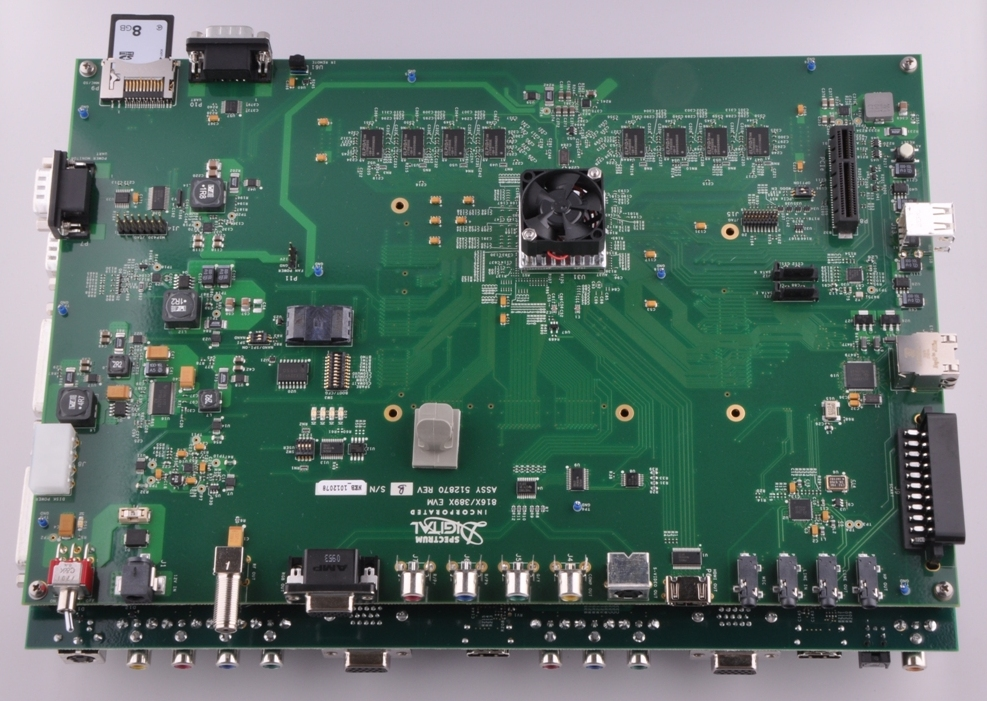
\includegraphics[scale=0.4]{../Pictures/top_ti816x_evm.png}
	\caption{Draufsicht auf das EVM8168}
	\label{fig:top_ti816x_evm}
\end{figure}



\section{Der DaVinci\texttrademark}\label{sec:davinci}
Bei dem auf dem EVM816x verwendeten ARM-Prozessor DM816x handelt es sich um einen eigentlich f�r die Videoprozessierung optimierten Prozessor der DaVinci\texttrademark-Familie von Texas Instruments.\\
Der DM816x ist ein heterogener Prozessor, der mehreren Subsystemen und Coprozessoren besteht.
Genauer gibt des folgende Subsysteme:

\begin{itemize}
\item ARM Subsystem mit einem Cortex-A8 der Firma ARM (\textbf{\ref{subsec:a8}})
\item DSP Subsystem mit einem C674x VLIW DSP der Firma Texas Instruments (\textbf{\ref{subsec:dsp}})
\item SGX530 3D Grafik Engine
\item 512kb On-Chip RAM
\item High-Definition Video Image Coprozessoren (HDVICP2)
\item Media Controller
\item HD Video Processing Subsystem (HDVPSS)
\item System Control
\item Peripherie
\end{itemize} 

All diese Subsysteme und Coprozessoren sind durch eine gemeinsame System Interconnection miteinander verbunden. \textbf{Abbildung \ref{fig:dm8168}} zeigt das funktionale Blockdiagramm des DM816x.\\
%
\begin{figure}[htbp]
	\centering
		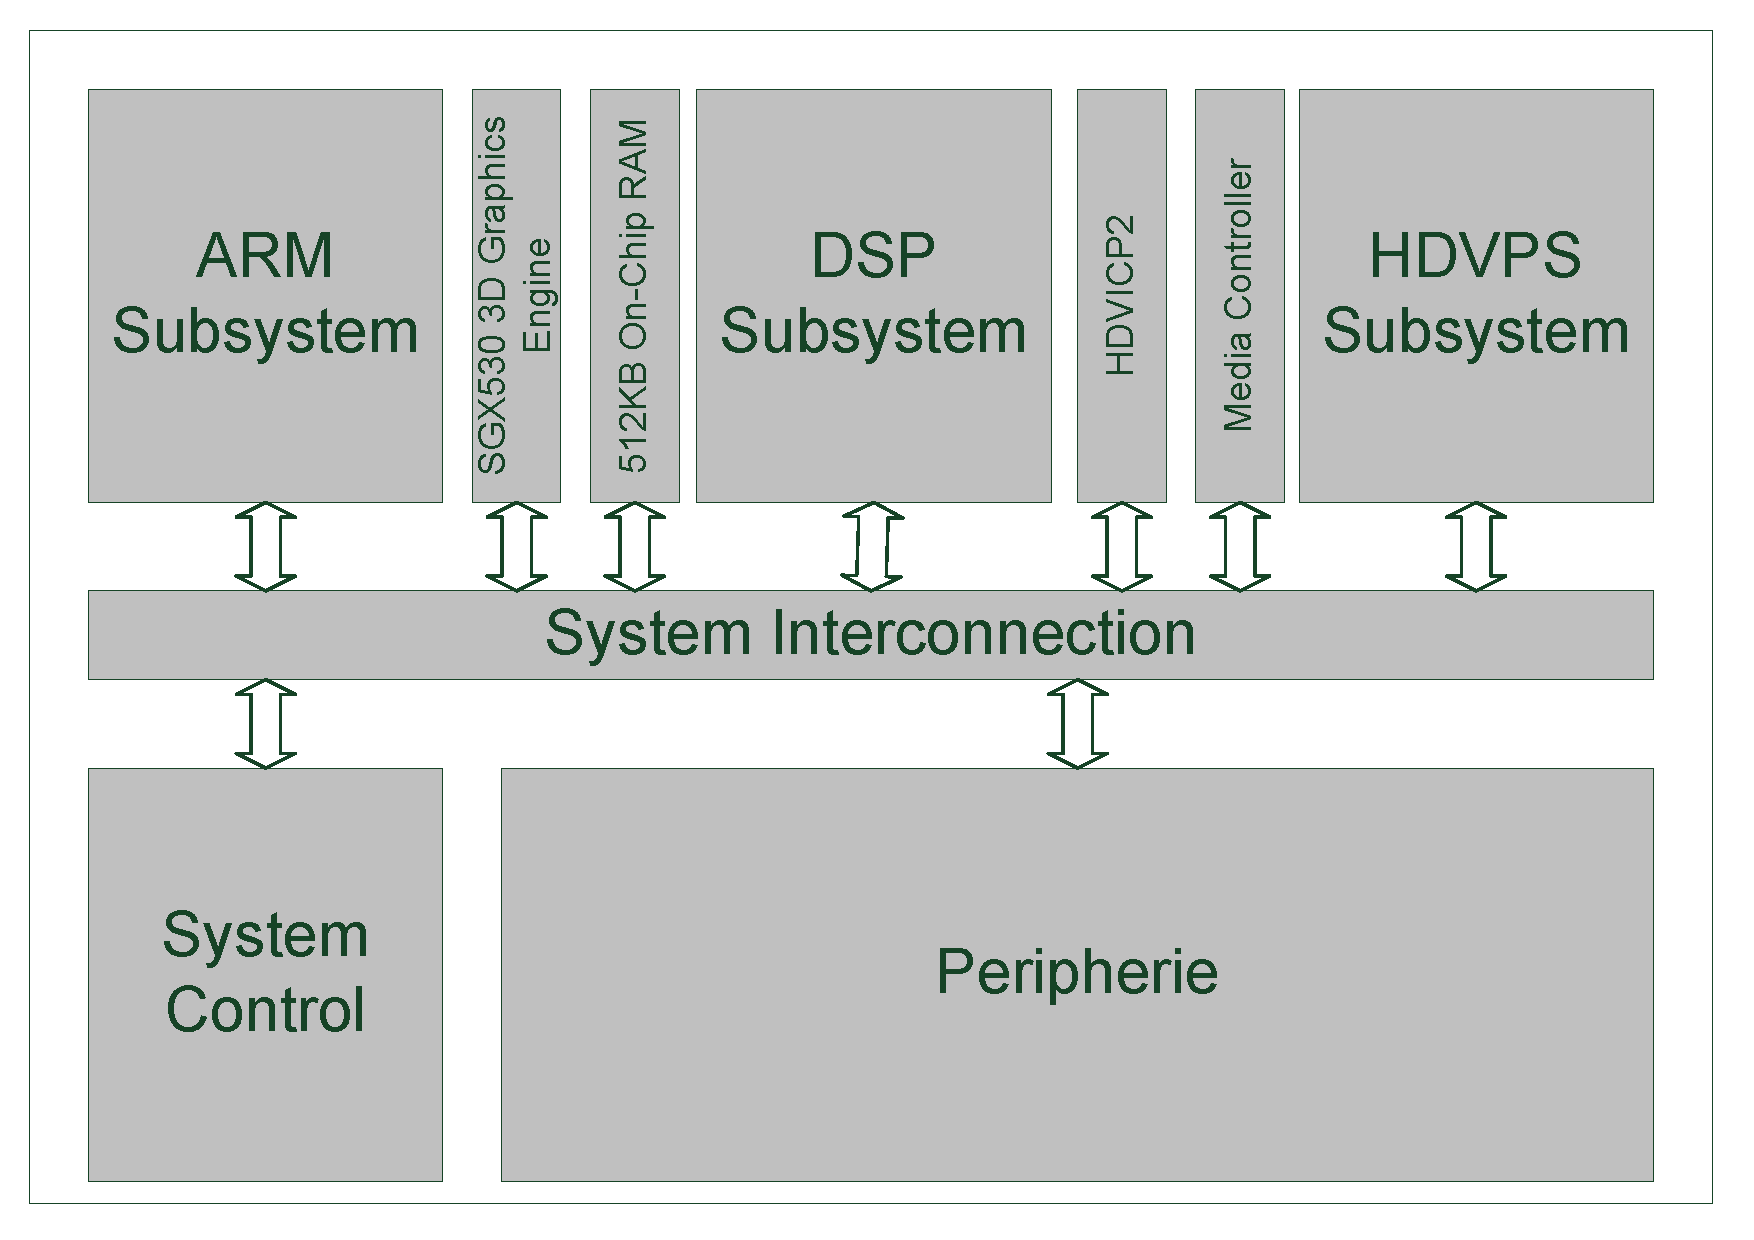
\includegraphics[scale=0.5]{../Pictures/dm8168.pdf}
	\caption{Funktionales Blockdiagramm des DM816x\cite{evm8168}}
	\label{fig:dm8168}
\end{figure}
%

\subsection{ARM Cortex-A8}\label{subsec:a8}

Der erste Prozessor aus der heterogenen Prozessorarchitektur des DM8168 der vorgestellt werden soll, ist ein Cortex-A8 der Firma ARM. Hierbei handelt des sich um einen General-Purpose Prozessor im RISC Design. Er besteht im wesentlichen aus 6 Komponenten (vgl. \textbf{Abbildung \ref{fig:a8}}):

\begin{itemize}
	\item Instruction Fetch
	\item Instruction Decode
	\item Instruction Execute
	\item Load/Store
	\item L2 Cache
	\item NEON-Coprozessor (\textbf{\ref{subsubsec:neon}})
\end{itemize}
%
\begin{figure}[h]
	\centering
		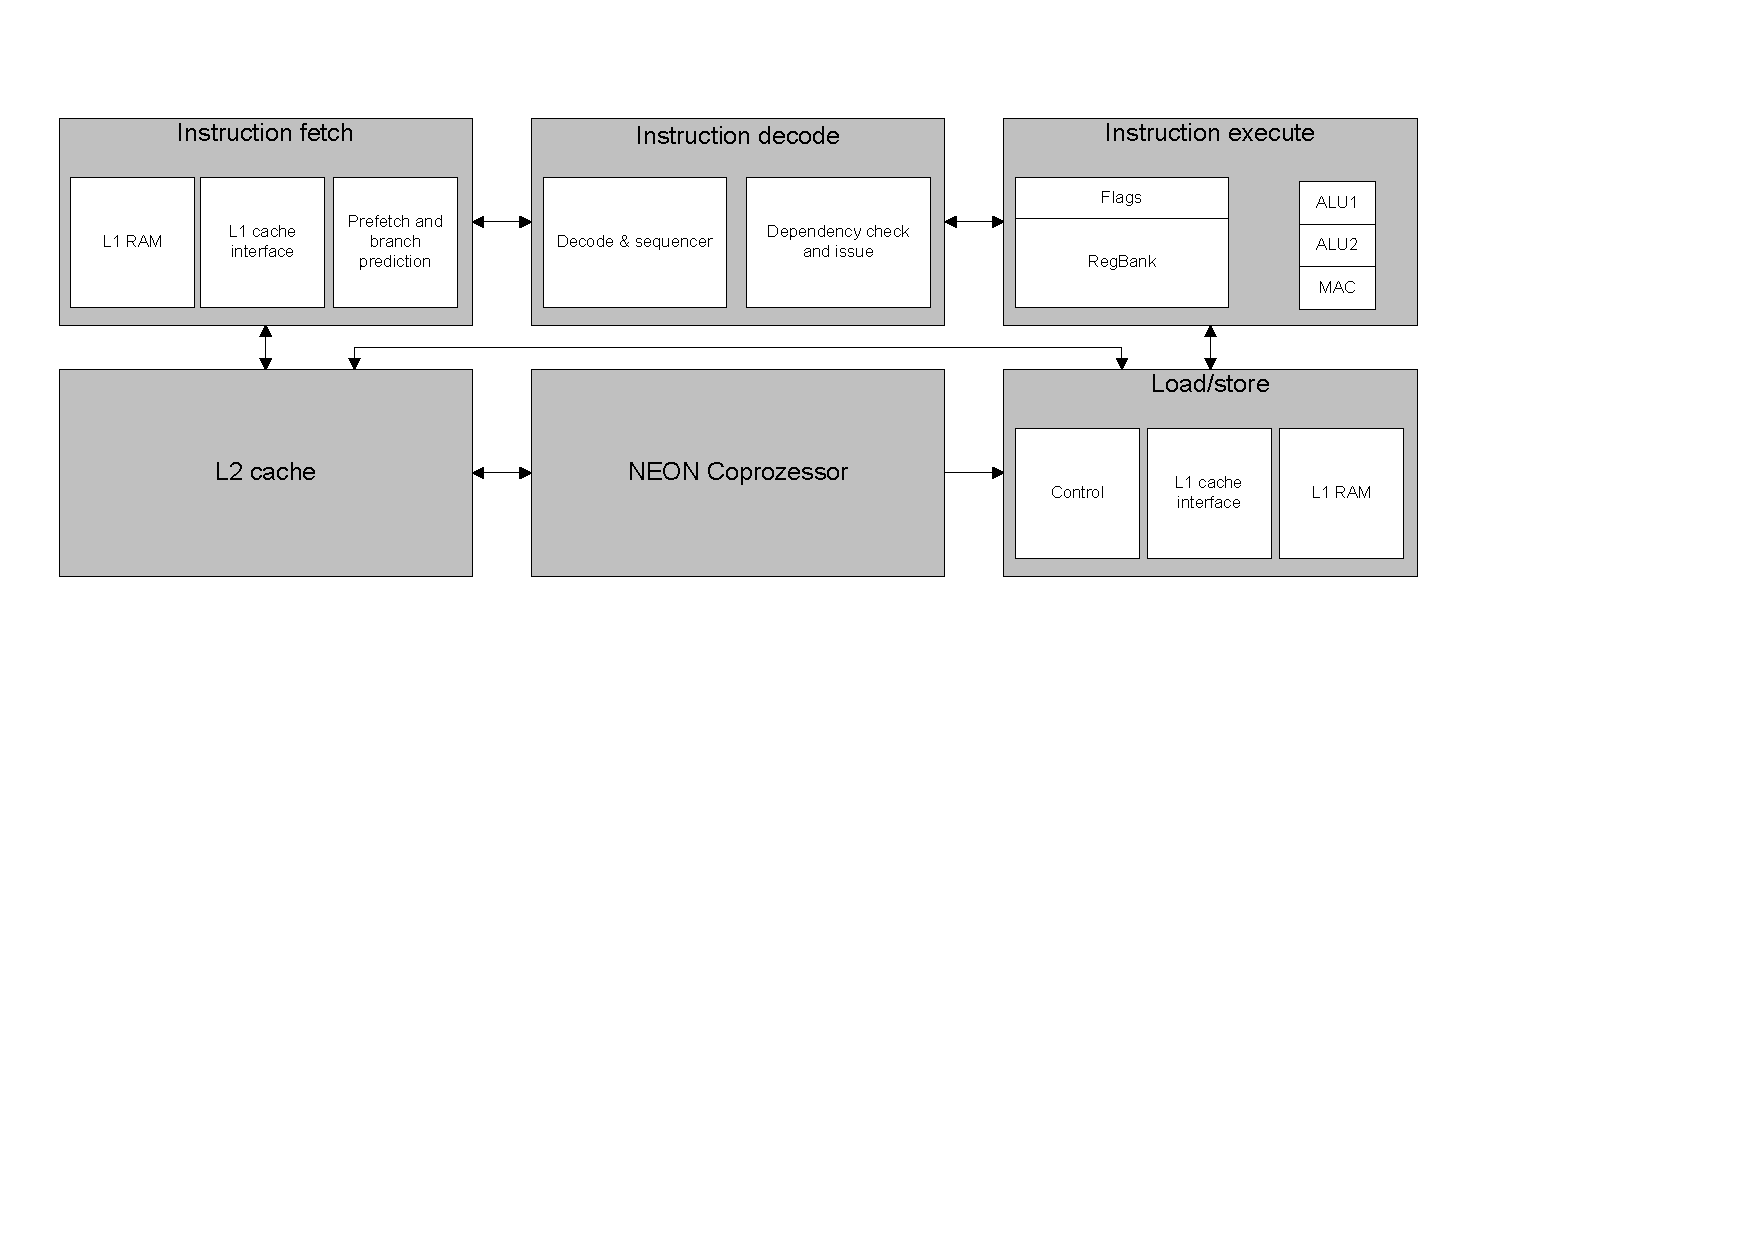
\includegraphics[width=1\textwidth]{../Pictures/cortexa8.pdf}
	\caption{Cortex-A8 Blockdiagramm\cite{cortexa8}}
	\label{fig:a8}
\end{figure} 
%
Wie in der Abbildung zu sehen ist, besteht der Cortex-A8 aus zwei wesentlichen Teilen:
\begin{itemize}
\item ARMv7 Prozessorkern (\textbf{\ref{subsubsec:armv7}})
\item NEON-Coprozessor (\textbf{\ref{subsubsec:neon}})
\end{itemize}

Diese beiden Prozessorkerne teilen sich Instruction Fetch, Instruction Decode, Instruction Execute, Load/Store und L2 Cache.\\

\subsubsection{ARMv7-A Prozessorkern}\label{subsubsec:armv7}
Der ARMv7-A Prozessorkern besitzt neben Operationen f�r Spr�nge, etc. nur Operationen f�r die Berechnung von Integerwerten.\\
Die Caches dieses Prozessorkerns besitztem folgende Eigenschaften:
\begin{itemize}
\item separate L1 Instruktions- und Datencaches
\begin{itemize}
\item Harvard Architektur
\item Gr��e von 32 KB
\item 64 Bytes Zeilenl�nge
\item vierfach assoziative Cachestruktur
\end{itemize}
\item L2 Cache
\begin{itemize}
\item Gr��e von 256KB
\item 64 Bytes Zeilenl�nge
\item achtfach assoziative Cachestruktur
\end{itemize}
\end{itemize}
Instruktionen werden in einer dreiphasigen Pipeline abgearbeitet, die wiederum in 13 Stufen unterteilt ist.\\
Die Fetch-Phase besitzt drei Stufen. In ihr werden ben�tigte Befehle aus dem L1-Instruction-Cache geladen, der sich in der Instruction Fetch-Einheit befinden (vgl. \textbf{Abbildung \ref{fig:a8}}).\\
Diese Instruktionen werden in einen Buffer geladen, welcher in der Decode-Phase, welche in f�nf Stufen unterteilt ist, ausgelesen wird und die Instruktionen decodiert werden. Au�erdem wird in der Decode-Phase die Ausf�hrungsreihenfolge der geladenen Befehle festgelegt. Diese Reihenfolge h�ngt von Datenabh�ngigkeiten und Ausf�hrungszeiten der einzelnen Operationen ab, die f�r die Ausf�hrung ben�tigt werden (eine �bersicht der Instruktionen wird im Anhang gegeben).\\
In der Execute-Phase werden anschlie�end die Befehle an die entsprechenden Funktionseinheiten weitergeleitet. Dieses geschieht in sechs Stufen.\\
Wie schon erw�hnt ist dieser Prozessorkern auf Integeroperationen ausgelegt, wird aber bei der Kompilierung eines Programms f�r den Cortex-A8 dem Compiler nicht die Benutzung einer Floating Point-Einheit vorgeschrieben (vgl. \textbf{Kapitel \ref{subsubsec:neon}}) werden auch entsprechende Befehle auf den Integeroperationen des ARMv7-A Prozessorkerns emuliert, was zu langen Ausf�hrungszeiten f�hren kann. Derartige Floating Point Instruktionen sind durch das Pr�fix \textit{\_\_aeabi\_} im Assembler-Code gekennzeichnet. Dieses bedeutet, dass Floating Point-Operationen nicht auf Hardware-, sondern auf Softwareebene berechnet werden.\\
Die \textbf{Tabelle \ref{tab:aeabi}} gibt einen �berblick �ber die in Software hinterlegten Floating Point-Operationen des ARMv7 Prozessorkerns.\\
%
\begin{table}[h]
\centering
\begin{tabular}{|c|c|}
\hline
Befehl & Beschreibung\\
\hline\hline
float \_\_aeabi\_fadd(float a, float b) & single-precision Addition\\
float \_\_aeabi\_fdiv(float n, float d) & single-precision Division, n/d\\
float \_\_aeabi\_fmul(float a, float b) & single-precision Multiplikation\\
float \_\_aeabi\_frsub(float x, float y) & single-precision umgekehrte Subtaktion, y - x\\
float \_\_aeabi\_fsub(float x, float y) & single-precision Subtraktion, x - y\\
int \_\_aeabi\_fcmpeq(float a, float b) & 1, wenn a = b\\
int \_\_aeabi\_fcmplt(float a, float b) & 1, wenn a < b\\
int \_\_aeabi\_fcmple(float a, float b) & 1, wenn a <= b\\
int \_\_aeabi\_fcmpge(float a, float b) & 1, wenn a >= b\\
int \_\_aeabi\_fcmpgt(float a, float b) & 1, wenn a > b\\
\hline
\end{tabular}
\caption{Auszug der Floating Point-Operationen des ARMv7\cite{aeabi}}
\label{tab:aeabi}
\end{table}
%
Der Instruktionssatz des ARMv7-A Prozessorkerns besitzt des weiteren Operationen die f�r die Kommunikation zwischen ihm und angeschlossenen Coprozessoren benutzt werden k�nnen. Diese Funktionen werden mir MCR und MRC bezeichnet und weisen je nach angesprochenem Coprozessor unterschiedliche Ausf�hrungszeiten auf, diese Operationen ben�tigen aber immer mindestens 60 Takte.

\subsubsection{Der NEON-Coprozessor}\label{subsubsec:neon}
Dieser Coprozessor beherbergt zwei Einheiten zur Berechnung von Floating Point-Operationen. Zum Einen ist das die VFPv3-Einheit (\textbf{\ref{ph:vfp}}) und zum Anderen die NEON-SIMD-Einheit (\textbf{\ref{ph:neon}}). 
%
\begin{figure}[h]
	\centering
		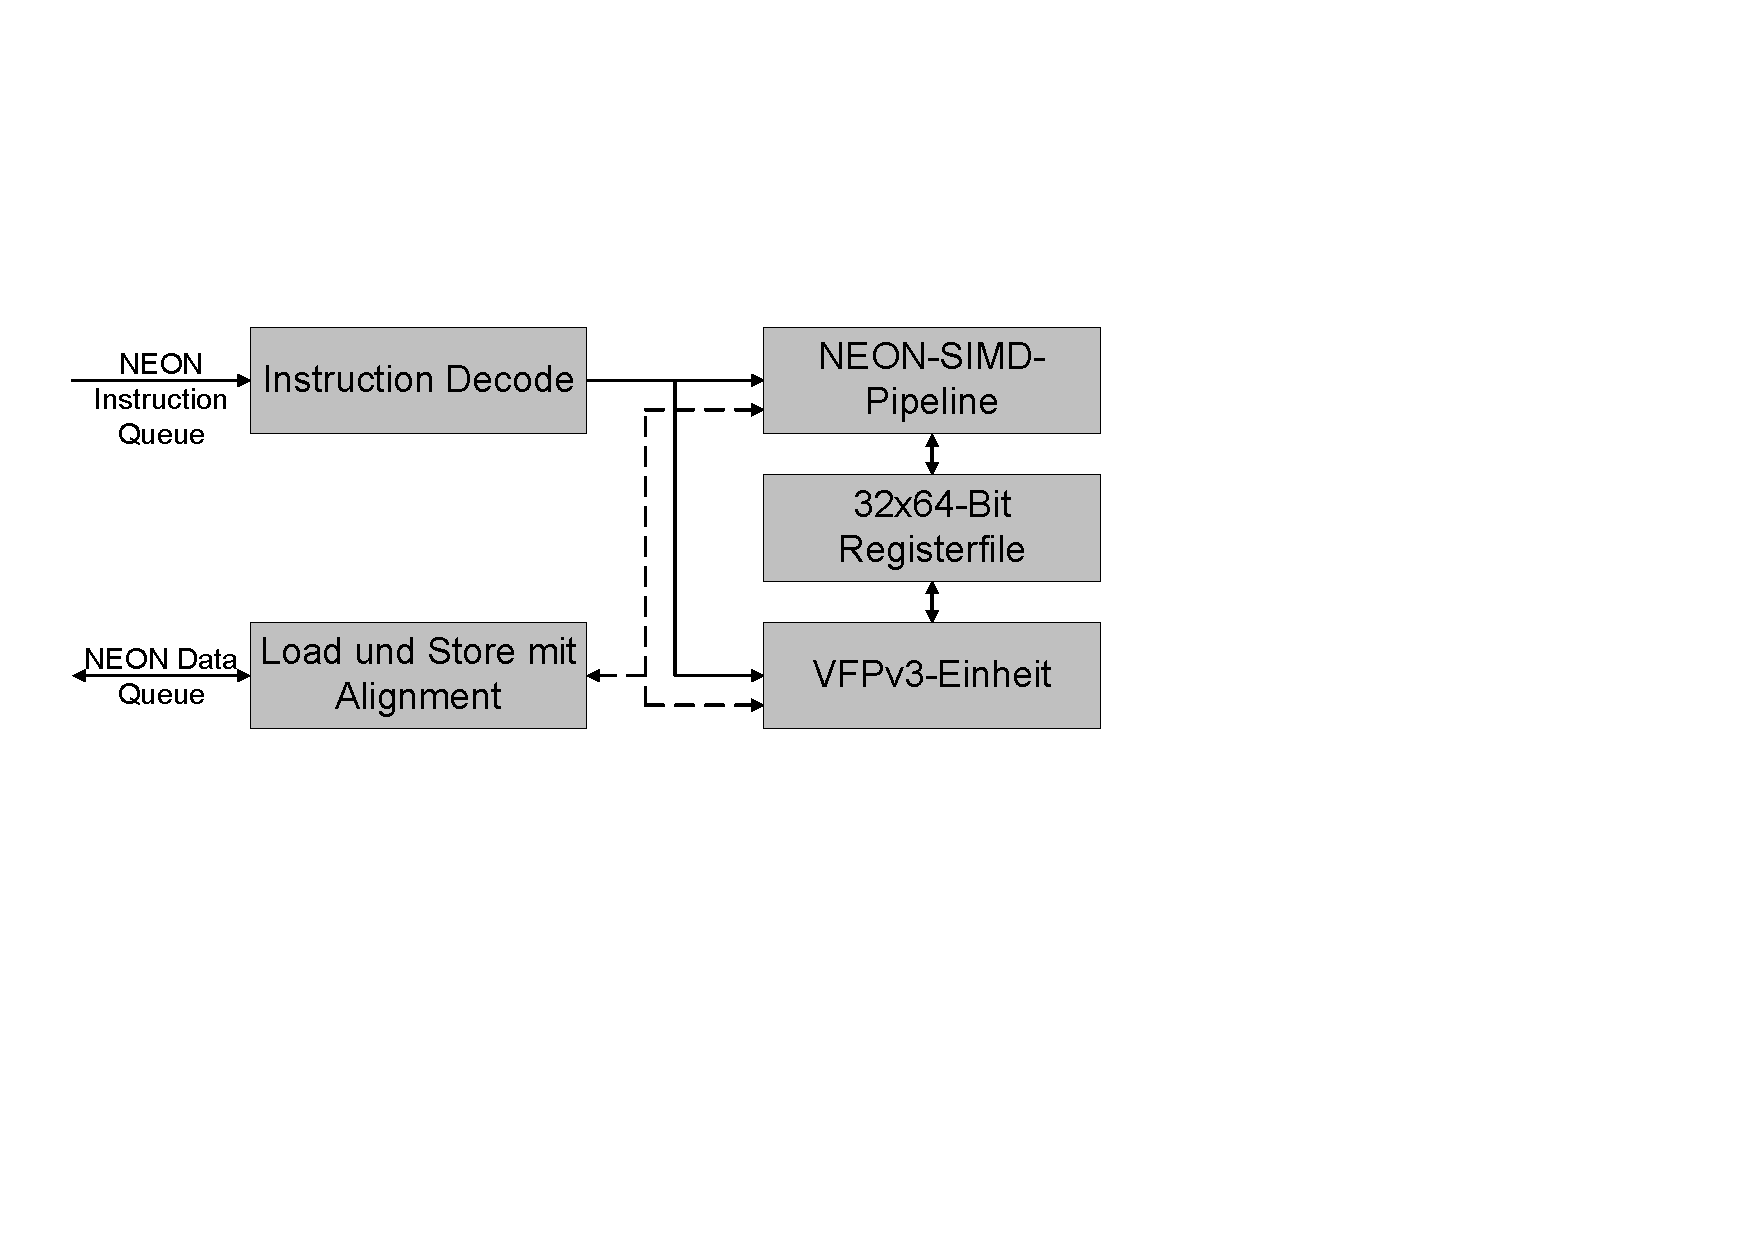
\includegraphics[scale=0.8]{../Pictures/NEON.pdf}
	\caption{Vereinfachtes Blockdiagramm des NEON-Coprozessors}
	\label{fig:neon}
\end{figure} 
%

Des weiten sind noch:
\begin{itemize}
\item Eine NEON-Registerbank mit 32x64-bit General-purpose Registern,
\item eine NEON Integer Execute Pipeline (ALU,Shift,MAC),
\item eine NEON Double- und Single-Precision Floating Point Execute Pipeline (FADD, FMUL)
\item und eine NEON Load/Store und Permute Pipeline vorhanden.
\end{itemize}
Die 32x64-bit Register liegen in einer Registerbank, die unabh�ngig von der Registerbank des ARMv7 Prozessorkerns ist, \textbf{Abbildung \ref{fig:neonbank}} zeigt die Sicht von der VFPv3- und der NEON-SIMD-Einheit auf dieses Register.\\
%
\begin{figure}[h]
	\centering
		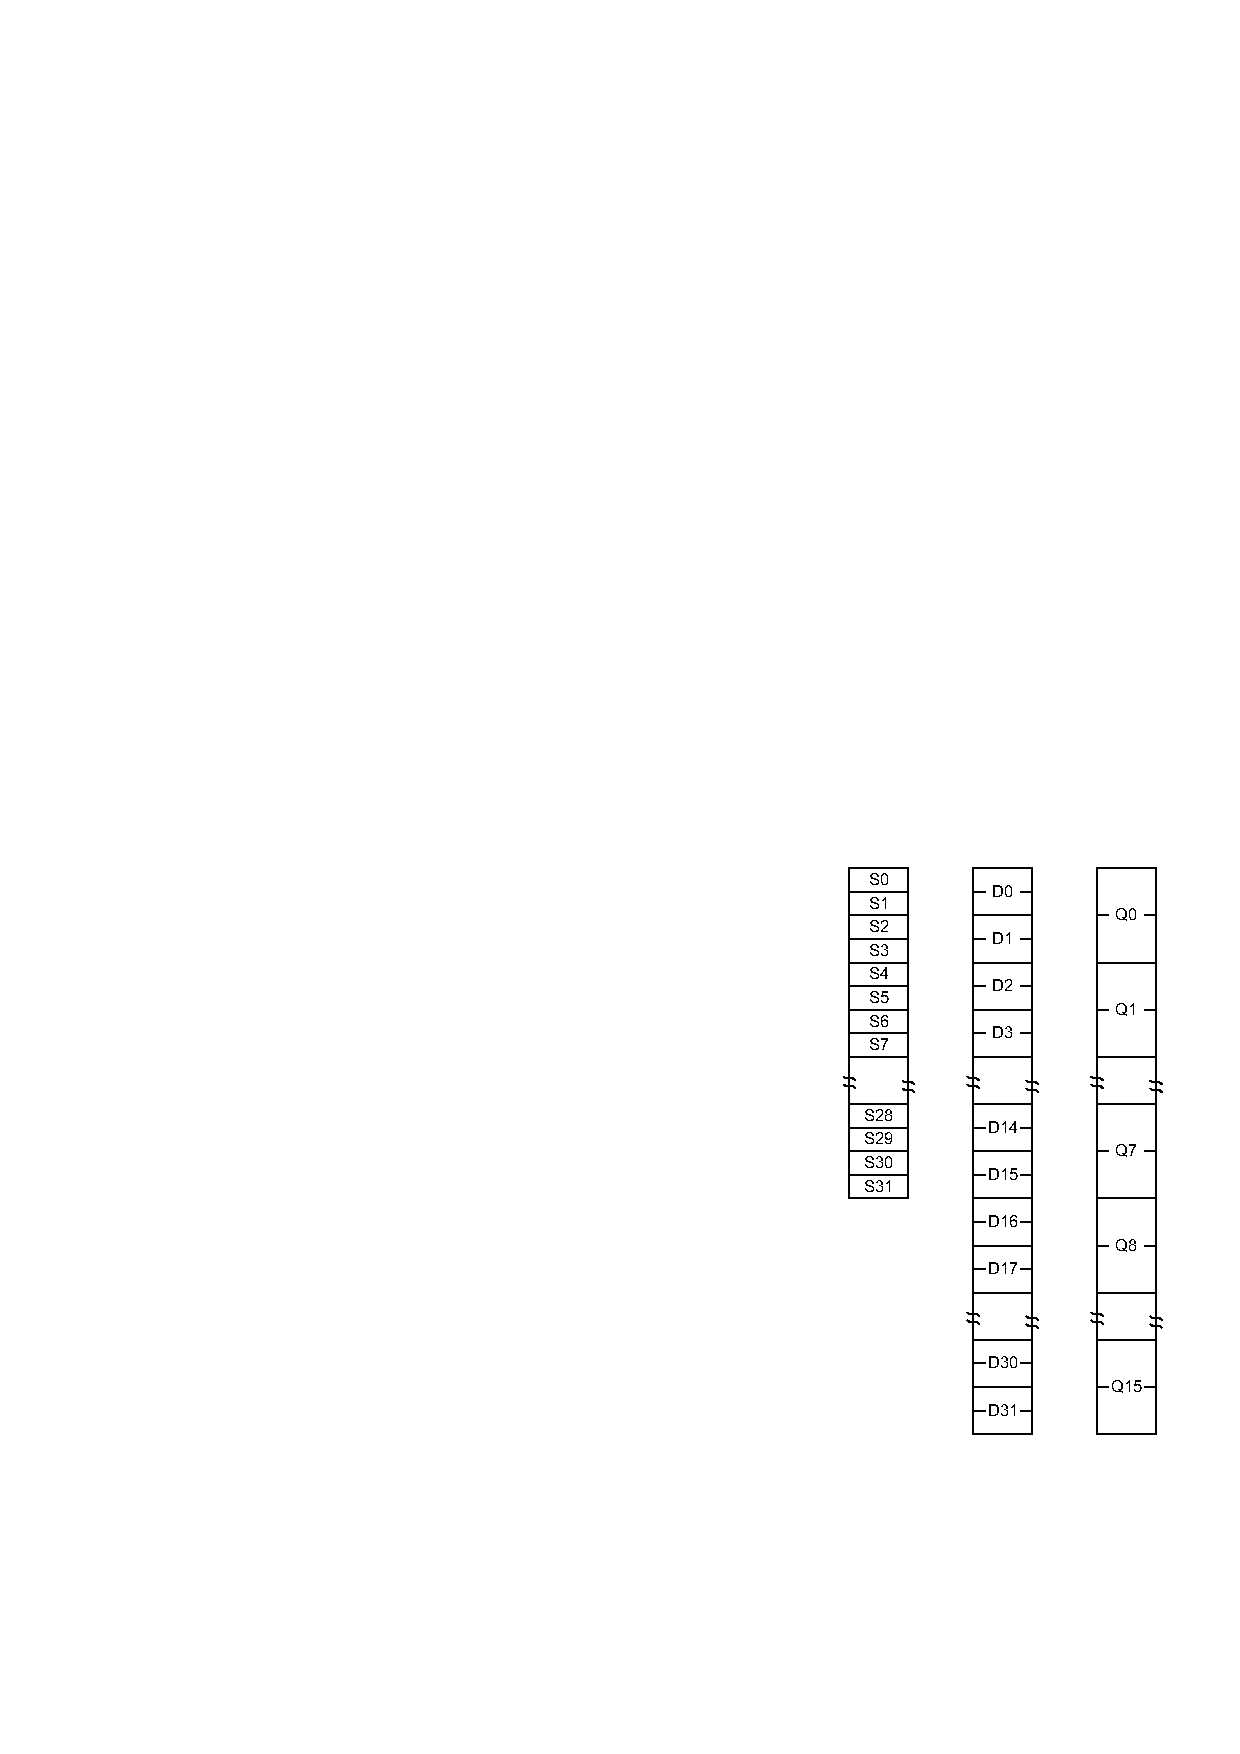
\includegraphics[scale=0.8]{../Pictures/neonbank.pdf}
	\caption{Register der NEON-SIMD- und der VFPv3-Einheit\cite{cortexa8}}
	\label{fig:neonbank}
\end{figure} 
%
Die Kommunikation zwischen ARM und NEON-Einheit geschieht l�sst sich in zwei Teile unterteilen:
\begin{itemize}
\item Weiterleitung von Befehlen
\item Weiterleitung von Daten
\end{itemize}

Die Weiterleitung von Befehlen vom ARM zum NEON-Coprozessor geschieht in folgenden Schritten:

\begin{enumerate}
\item NEON-SIMD- und VFPv3-Befehle durchlaufen die gesamte ARM-Pipeline und werden am Ende der Execute-Phase in eine NEON Instruction Queue geladen, welche 16 Eintr�ge halten kann. Danach gelten die NEON- und VFPv3-Befehle als abgearbeitet und er kann wieder ARM-Befehle ausf�hren. Eine Ausnahme bildet hier der Fall, dass die 
\item Der NEON-Coprozessor lie�t aus dieser Queue und muss die Befehle nochmals Dekodieren und ihre Abarbeitungsreihenfolge festlegen NEON Instruction Queue voll ist. Sollte dieses geschehen muss der ARM warten bis wieder Eintr�ge in diese Queue geschrieben werden k�nnen.
\item Die NEON-SIMD- und VFPv3-Befehle werden auf dem NEON-Coprozessor verarbeitet
\item Mit dem MRC-Befehl lie�t der ARM die Ergebnisse des NEON-Coprozessors aus, dieses dauert mindestens 20 Takte
\end{enumerate}

Die Weiterleitung von Daten an den NEON-Coprozessor kann auf zwei Arten geschehen:

\begin{itemize}
\item Der ARM Prozessor schreibt mit dem MCR-Befehl Daten in die NEON Daten Queue, welch e12 Eintr�ge halten kann
\item oder der NEON-Coprozessor lie�t direkt aus dem L2 Cache.
\end{itemize}

Obwohl sich die NEON- und die VFP3-Einheit einige Befehle und die Registerbank teilen, haben sie doch entscheidende Unterschiede, die in den beiden folgenden Kapiteln erl�utert werden sollen.

\paragraph{VFPv3-Einheit}\label{ph:vfp}$\;$ \\\\
Die VFPv3-Einheit stellt einen Coprozessor, welcher auf der \textit{VFPv3-Architektur} basiert, zur Berechnung von Floating Point-Zahlen zur Verf�gung und unterst�tzt den \textit{ANSI/IEEE Standard 754-1985} in vollem Umfang.\\
Hierf�r stellt die VFPv3-Einheit Operationen zur Addition, Subtraktion, Multiplikation, Division, Multiply-and-Accumulate und zur Wurzelberechnung zur Verf�gung, die sowohl mit Single-Precision als auch Double-Precision berechnet werden k�nnen. Des weiteren werden Operationen zur Konvertierung zwischen Floating- und Fix-Point und Floating-Point und Konstanten bereitgestellt.\\
Die VFPv3-Einheit besitzt keine Pipeline-Struktur und ist nur in der Lage Anweisungen sequenziell abzuarbeiten.\\
Sie hat auf die in \textbf{Abbildung \ref{fig:neonbank}} abgebildete Registerbank Zugriff wie folgt:

\begin{itemize}
\item Als 32 32-bit Einzelwortregister, S0-S31, in dieser Sicht ist nur die halbe Registerbank zugreifbar,
\item Als 32 64-bit Doppelwortregister, D0-D31
\item und als Kombination dieser 32- und 64-bit Register
\end{itemize}

In \textbf{Tabelle \ref{tab:vfp}} sind wesentliche Instruktionen aus dem Instruktionssatz der VFPv3-Einheit mit Angabe der Ausf�hrungszeit in Takten gegeben. Hierbei ist zu erw�hnen, dass diese Ausf�hrungszeiten datenabh�ngig sind.

\begin{table}
\centering
\begin{tabular}{|c|c|c|}
\hline
Befehl & Single-Precision-Takte & Double-Precision-Takte\\
\hline\hline
FADD & 9-10 & 9-10\\
FSUB & 9-10 &9-10\\
FMUL \& FNMUL & 10-12 & 11-17\\
FMAC \& FNMAC & 18-21 & 19-26\\
FDIV & 20-37 & 29-65\\
FSQRT & 19-33 & 29-60\\
FABS & 4 & 4\\
FCMP & 4 oder 7 & 4 oder 7\\
FCPY & 4 & 4\\
\hline
\end{tabular}
\caption{Auszug aus dem Instruktionssatz der VFPv3-Einheit\cite{cortexa8}}
\label{tab:vfp}
\end{table}

\paragraph{NEON-SIMD-Einheit}\label{ph:neon}$\;$ \\\\
Die NEON-SIMD-Einheit ist eigentlich f�r die Ausf�hrung von Integeroperationen konzipiert, kann aber ebenfalls Floating Point-Operationen ausf�hren.\\
Diese Einheit basiert auf der \textit{Advanced SIMD Media Processing-Architektur}. SIMD steht hierbei f�r \textit{Single Input Multiple Data} und hei�t, dass ein und der selbe Befehle gleichzeitig auf mehrere Eingangsdaten angewendet werden kann. Der NEON-SIMD-Einheit ist es m�glich pro Operand 128 Bit gleichzeitig einzulesen und zu schreiben, allerdings kann sie nur 64 Bit gleichzeitig verarbeiten, woraus folgt, dass immer zwei Operationen parallel ausgef�hrt werden k�nnen.\\
Auch die NEON-SIMD-Einheit verwendet die in \textbf{Abbildung \ref{fig:neonbank}} abgebildete Registerbank und kann Operationen auf dieser mit folgenden Ein- und Ausgaberegistern ausf�hren:

\begin{itemize}
\item Mit 16 128-bit Quadwortregistern, Q0-Q15,
\item mit 32 64-bit Doppelwortregistern,D0-D31, die auch von der VFPv3-Einheit sichtbar sind
\item und mit Kombinationen aus den 128- und 64-bit Registern.
\end{itemize}
Die Einheit kann bis zu zwei Advanced SIMD Operationen pro Takt von der Integer Execution Einheit des ARMs empfangen und zus�tzlich noch 32-bit MCR oder MRC Daten mit dieser tauschen.\\
Des weiten werden NEON-SIMD-Befehle in einer 10-stufigen Pipeline abgearbeitet.\\
Au�erdem ist es der NEON-SIMD-Einheit m�glich Teile der VFPv3-Befehle in ihrer Pipeline auszuf�hren um die Abarbeitungszeit zu beschleunigen.\\
In \textbf{Tabelle \ref{tab:neon}} ist ein Auszug des NEON-SIMD-Befehlssatzes mit Ausf�hrungszeiten in  Takten angegeben. Sigle-Precision-Befehle sind im sp�teren Assemblercode durch den Zusatz \textit{.f32} hinter dem Befehlsnamen gekennzeichnet.

\begin{table}[hpt]
\centering
\begin{tabular}{|c|c|c|}
\hline
Befehl & Takte\\
\hline\hline
VADD & 1-2\\
VSUB & 1-2\\
VMUL & 1-2\\
VABS & 1-2\\
VRSQRT&1-2\\
VMLA&1-2\\
VMLS&1-2\\
VMOV & 1\\
VLDR  & 1-2\\
VSTR  & 1-2\\
\hline
\end{tabular}
\caption{Auszug aus dem Floating Point-Befehlssatz der NEON-SIMD-Einheit\cite{cortexa8}}
\label{tab:neon}
\end{table}

\subsubsection{Ansteuerungsm�glichkeiten}
Wird beider Kompilierung nicht spezifiziert, wie Floating Point-Operationen behandelt werden sollen, werden diese immer mit den in \textbf{Tabelle \ref{tab:aeabi}} angegeben Softwarefunktionen emuliert.\\
Sollen solche Operationen auf der VFPv3-Einheit ausgef�hrt werden muss lediglich das Flag \textit{\-mfpu=vfp} gesetzt werden.\\
Die NEON-SIMD-Einheit kann auf den �blichen vier wegen Angesprochen werden:
\begin{itemize}
\item Ansteuerung durch den Compiler
\item Unterst�tzung des Compilers durch Umstrukturierung des Codes
\item Einf�gen von Intrinsics in den Code
\item Algorithmen direkt in NEON-Assembler schreiben
\end{itemize}
Da diese vier Optionen f�r die sp�tere Optimierung verwendet werden, soll zu jeder dieser Varianten auch noch ein Beispiel gegeben werden. Wichtig ist, dass bei allen vier Varianten das Compilerflag \textit{-mfpu=neon} gesetzt sein muss.
 
\paragraph{Compiler}\label{ph:neoncomp}$\;$ \\\\
Die erste Variante ist die am leichtesten Umzusetzende. Hierbei wird nur das vorher erw�hnte Compilerflag gesetzt und der Compiler f�gt w�hrend der Kompilierung an ihm sinnvoll erscheinenden Stellen NEON-Assembler-Code ein.\\
Als Beispiel soll hier ein einfacher Beipielcode verwendet werden der in den \textbf{Listings \ref{code:spfc} - \ref{code:spfneon}} in C, ARM-Assembler und in ARM+NEON-Assembler angegeben wird.

\begin{lstlisting}[caption=1. einfaches Beispiel in C, label=code:spfc]
 int i;
 for (i = 0; i < 200; i++) {
 z[i] = a[i] * b[i];
 }
\end{lstlisting}

\begin{lstlisting}[caption=ARM-Assembler, label=code:spfarm]
	PUSH     {r4,r5,lr}
	MOV      r3,#0
|L1.8|:
	ADD      r4,r0,r3,LSL #1
	ADD      r5,r1,r3,LSL #1
	LDRH     r4,[r4,#0]		;Laden von a[i];
	LDRH     r5,[r5,#0]		;Laden von b[i];
	SMULBB   r4,r4,r5
	ADD      r5,r2,r3,LSL #1
	ADD      r3,r3,#1
	CMP      r3,#0xc8		;200 Iterationen;
	STRH     r4,[r5,#0]     ;Speichern in z[i];
	BLT      |L1.8|
	POP      {r4,r5,pc}
\end{lstlisting}

\begin{lstlisting}[caption=ARM+NEON-Assembler, label=code:spfneon]
	MOV      r3,#0x19 		;nur noch 25 Iterationen;
|L1.4|
	VLD1.16  {d0,d1},[r0]!	;Laden von a;
	SUBS     r3,r3,#1
	VLD1.16  {d2,d3},[r1]!  ;Laden von b;
	VMUL.I16 q0,q0,q1		;a*b;
	VST1.16  {d0,d1},[r2]!	;Speichern in z;
	BNE      |L1.4|
	BX       lr
\end{lstlisting}

Hierbei sieht man, dass sowohl die Lade und Speicheroperationen, als auch, dass die Multiplikation an sich parallelisiert wurden.

\paragraph{C-Code}\label{ph:neonc}$\;$ \\\\
Die zweite Variante erfordert ein Eingreifen in die Code-Struktur. Hierbei geht es darum, kritische Stellen im Code zu identifizieren und zu isolieren, die es dem Compiler nicht erlauben eine auf den NEON abbildbare Codestelle zu erkennen. Dieses kommt insbesondere bei verschachtelten Anweisungen und bei unklaren Datenabh�nigikeiten vor.

\paragraph{Intrinsics}$\;$ \\\\
Eine weitere Variante bietet das Ersetzten von Berechnungen durch Intrinsics, die die entsprechende Berechnung auf Assembler-Ebene darstellen. Eine Liste der vorhandenen Intrinsics ist in \cite{intrinsics} zu finden.\\
Eine solche Ersetzung von Berechnungen durch Intrinsics soll an einem weiteren einfachen  Beispiel in den \textbf{Listings \ref{code:hamc} - \ref{code:hamneon}} verdeutlicht werden.

\begin{lstlisting}[caption=2. einfaches Beispiel in C, label=code:hamc]
	int i;
 	for(i=0;i<200;i++) {
 	z[i] = x[i] + y[i];
 	}
\end{lstlisting}

\begin{lstlisting}[caption=2. einfaches Beipiel mit Intrinsics, label=code:hamcv]
	int i;
	uint32x4_t x4,y4; // Hier werden 128 bit Register definiert, die die Operanten halten 
	uint32x4_t z4;    // Hier wird ein 128 bit Register definiert, dass das Ergebnis h�lt 
	uint32_t *ptra = x; //x,y und z sind die Eingangs-, bzw. Ausgangsarrays 
	uint32_t *ptrb = y; 
	uint32_t *ptrz = z; 

	for(i=0; i < 200/4; i++)
	{
        x4 = vld1q_u32(ptra);  // Intrinsic um x4 mit 4 Werten von x zu laden
        y4 = vld1q_u32(ptrb);  // Intrinsic um y4 zu laden
        z4=vaddq_u32(x4,y4);   // Intrinsic um z4=x4+y4 zu addieren
        vst1q_u32(ptrz, z4);   // Speicher die 4 Ergebnisse in z
        ptra+=4; // Pointer inkrementieren
        ptrb+=4;
        ptrz+=4;
	}
\end{lstlisting}

\begin{lstlisting}[caption=ARM+NEON-Assembler, label=code:hamneon]
        add      r3, r1, #800
.L2:
        vld1.32  {d4-d5}, [r1] ;Zeile 10;
        add      r1, r1, #16
        vld1.32  {d6-d7}, [r0] ;Zeile 11;
        cmp      r1, r3
        vadd.i32 q3, q3, q2    ;Zeile 12;
        vst1.32  {d6-d7}, [r2] ;Zeile 13;
        add      r0, r0, #16
        add      r2, r2, #16
        bne      .L2
        bx       lr
\end{lstlisting}

In \textbf{Listing \ref{code:hamneon}} sind alle Instruktionen wiederzufinden, die in \textbf{Listing \ref{code:hamcv}} definiert wurden.

\paragraph{Assembler}\label{ph:neonasm}$\;$ \\\\
Als letzte Variante soll die direkte Umsetzung einer Berechnung in NEON-Assembler vorgestellt werden. Hierbei werden einzelne Methoden oder ganze Programmteile nicht in einer Hochsprache wie C/C++ geschrieben sondern in NEON-Assembler.\\
Als Beispiel soll hier eine Methode aus der FFT der Libav-Bibliothek angef�hrt werden. Die Libav-Bibliothek wird im Optimierungskapitel vorgestellt.\\
Die \textbf{Linstings \ref{code:fft4c}} und \textbf{\ref{code:fft4neon}} zeigen einmal die Methode \textit{FFT4} in C-Code und in NEON-Assembler.

\begin{lstlisting}[caption= FFT4 in C, label=code:fft4c]
static void fft4(FFTComplex *z)
{
#define BF(x, y, a, b) do {                     \
        x = a - b;                              \
        y = a + b;                              \
    } while (0)

    FFTDouble t1, t2, t3, t4, t5, t6, t7, t8;

    BF(t3, t1, z[0].re, z[1].re);
    BF(t8, t6, z[3].re, z[2].re);
    BF(z[2].re, z[0].re, t1, t6);
    BF(t4, t2, z[0].im, z[1].im);
    BF(t7, t5, z[2].im, z[3].im);
    BF(z[3].im, z[1].im, t4, t8);
    BF(z[3].re, z[1].re, t3, t7);
    BF(z[2].im, z[0].im, t2, t5);
}
\end{lstlisting}

\begin{lstlisting}[caption=FFT4 in NEON-Assembler, label=code:fft4neon]
function fft4_neon
        vld1.32         {d0-d3}, [r0,:128]

        vext.32         q8,  q1,  q1,  #1       @ i2,r3 d3=i3,r2
        vsub.f32        d6,  d0,  d1            @ r0-r1,i0-i1
        vsub.f32        d7,  d16, d17           @ r3-r2,i2-i3
        vadd.f32        d4,  d0,  d1            @ r0+r1,i0+i1
        vadd.f32        d5,  d2,  d3            @ i2+i3,r2+r3
        vadd.f32        d1,  d6,  d7
        vsub.f32        d3,  d6,  d7
        vadd.f32        d0,  d4,  d5
        vsub.f32        d2,  d4,  d5

        vst1.32         {d0-d3}, [r0,:128]

        bx              lr
endfunc
\end{lstlisting}

Hierbei werden immer zwei Berechnungen parallel durchgef�hrt. Jedes BF() in \textbf{Listing \ref{code:fft4c}} besteht aus einer Addition und einer Subtraktion, es werden also insgesamt acht Additionen und 8 Subtraktionen durchgef�hrt. Im NEON-Assembler-Code aus \textbf{Listing \ref{code:fft4neon}} befinden sich vier VADDs und vier VSUBs, die jeweils f�r 2 parallele Berechnungen stehen. Also kommen wir auch hier wieder auf acht Additionen und acht Subtraktionen.

\subsection{Der C674x-DSP-Prozessor}\label{subsec:dsp}
Der C674x-DSP der Firma Texas Instruments geh�rt zur C6000-Familie und ist VLIW DSP mit Floating Point-Hardware. \textbf{Abbildung \ref{fig:DSPblock}} zeigt das Blockdiagramm des DSPs.
%
\begin{figure}[h]
	\centering
		\includegraphics[width=1\textwidth]{../Pictures/DSPblock.pdf}
	\caption{C674x Blockdiagramm\cite{evm8168}}
	\label{fig:DSPblock}
\end{figure} 
%
\subsubsection{Hardware}
Aus \textbf{Abbildung \ref{fig:DSPblock}} lassen sich folgende Hardwarekomponenten entnehmen:
\begin{itemize}
\item C674x+ CPU
\item 32kB L1 Programm (L1P) RAM und Cache (bis zu 32kB) mit Error Detection Code (EDC)
\item 32kB L1 Daten (L1D) RAM und Cache (bis zu 32kB)
\item 256kB zusammenh�ngender L2 RAM und Cache mit Error Correction Code (ECC)
\item External Memory Controller (EMC)
\item Interleaving Domain Multiple Access (IDMA)
\end{itemize}

Die Registerarchitektur innerhalb der C674x+ CPU, ihr Instruktionssatz und die Pipelinestruktur soll im Nachfolgenden n�her erl�utert werden.

\paragraph{Registerarchitektur und Instruktionssatz}\label{ph:reginst}$\;$ \\\\
Wie ebenfalls in \textbf{Abbildung \ref{fig:DSPblock}} zu sehen ist, besitzt die C674x+ CPU zwei parallele Datenpfade, die mit Register File A und B bezeichnet sind. Beide Datenpfade sind mit je mit einer 64 Bit-Leitung an den L1D-Cache angeschlossen, k�nnen also parallel 64 Bit lesen oder schreiben.\\
Innerhalb dieser Datenpfade befinden sich acht Ausf�hrungseinheiten zur Bearbeitung von Befehlen, je vier pro Datenpfad. Jeder Ausf�hrungseinheit ist hierbei ein Teil des Instruktionssatzes zugeordnet.\\
Daraus folgt, dass im Idealfall acht Befehle parallel pro Takt ausgef�hrt werden k�nnen.\\
\textbf{Abbildung \ref{fig:Register}} zeigt den Aufbau der beiden Datenpfade Register File A und B, nicht eingezeichnet sin die beiden sogenannten Crosspaths, die es Operationen aus dem Datenpfad A erlauben ein Datum pro Takt aus Register File B zu lesen und umgekehrt. Diese Crosspaths sind im Assembler-Code durch ein X hinter der Ausf�hrungseinheit gekennzeichnet.Insgesamt besitzt der DSP 64 32 Bit-Register, je 32 in A und B.
Auch wenn einige Befehle auf mehreren Ausf�hrungseinheiten ausgef�hrt werden k�nnen, lassen sich sich diese wie folgt grob unterteilen: 
\begin{itemize}
\item .M f�hrt Multiplikationen aus,
\item .L und .S sind prim�r alle anderen arithmetischen Operationen zust�ndig
\item und .D ist prim�r f�r das Laden und Speichern von Daten verantwortlich. 
\end{itemize}
%
\begin{figure}[h]
	\centering
		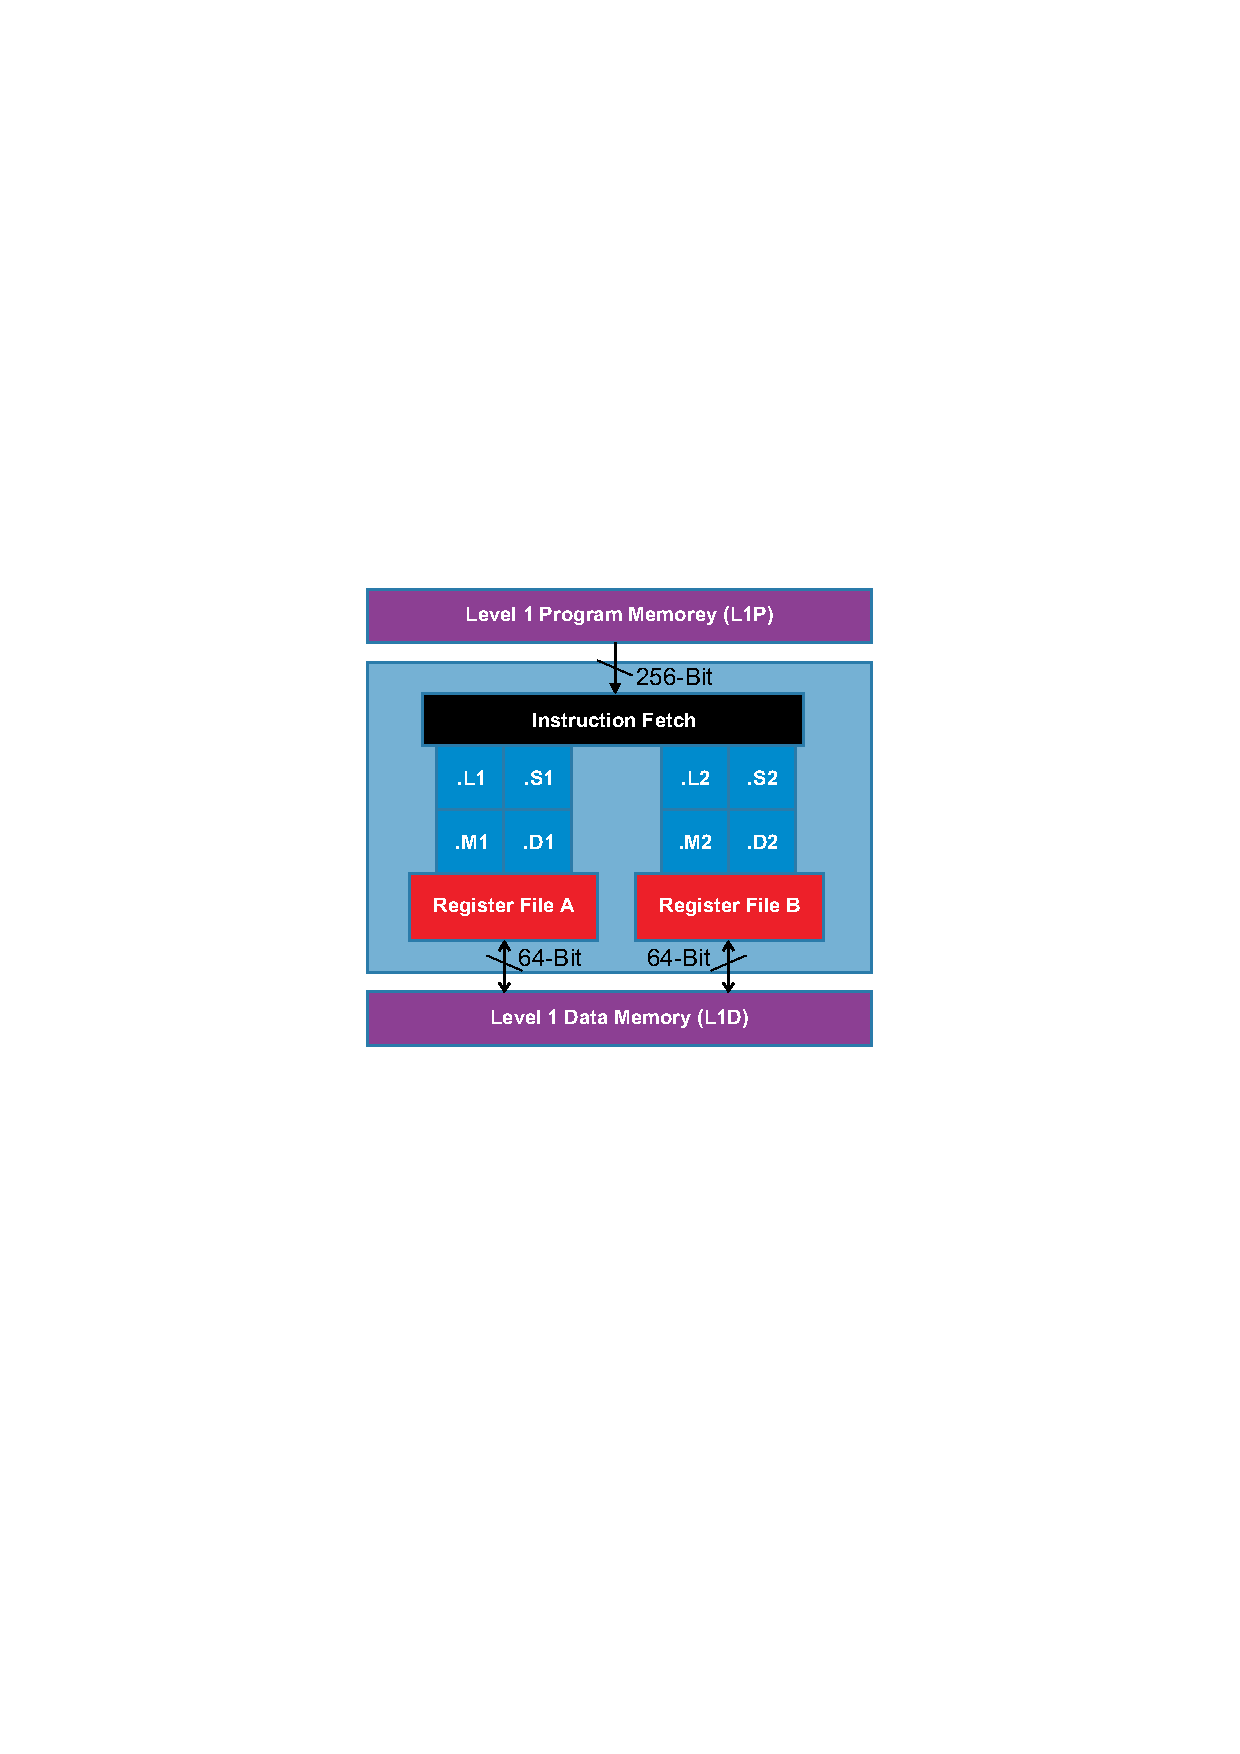
\includegraphics[scale=0.7]{../Pictures/Register.pdf}
	\caption{Stuktur der parallelen Datenpfade des C674x\cite{sprabf2}}
	\label{fig:Register}
\end{figure} 
%
\textbf{Tabelle \ref{tab:c674x}} gibt einen �berlick �ber die vorhandenen Befehle, in welcher Gruppe sie liegen, wieviele Takte sie ben�tigen und ihrer  Functional Unit Latency (FUL) und Delayslots, welche f�rs Pipelining wichtig sind. Hierbei gibt die Functional Unit Latency die Anzahl an Takten an, die eine Einheit nach Abschluss einer Berechnung ben�tigt, bis sie eine neue Berechnung annehmen kann. Die Delayslots geben die Takte an, die zwischen Einlesen der Operanden und dem Abschluss der Berechnung vergehen. Der Instruktionssatz besitzt keine Befehle f�r Divisionen oder Wurzeloperationen. Diese werden nach dem Newton-Raphson-Verfahren in Software emuliert.

\begin{table}[ht]
\centering
\begin{tabular}{|c|c|c|c|c|}
\hline
Befehl & Gruppe & Takte & Delayslots & FUL\\
\hline\hline
ADD & .D,.L\&.S & 1 & 0 & 0\\
ADDSP & .L\&.S & 4 & 3 & 1\\
ADDDP & .L\&.S & 7 & 6 & 2\\
LDW & .D & 5 & 4 & 0\\
MPY & .M & 2 & 1 & 0\\
MPYSP & .M & 4 & 3 & 1\\
MPYSPDP & .M & 7 & 6 & 3\\
MPYSP2DP & .M & 5 & 4 & 2\\
MPYDP & .M & 10 & 9 & 4\\
RSQRSP & .S & 1 & 0 & 1\\
RSQRDP & .S & 2 & 1 & 1\\
SUB & .D,.L\&.S & 1 & 0 & 0\\
SUBSP & .L\&.S & 4 & 3 & 1\\
SUBDP & .L\&.S & 7 & 6 & 2\\
\hline
\end{tabular}
\caption{Auszug aus dem Instruktionssatzssatz des C674x\cite{sprufe8b}}
\label{tab:c674x}
\end{table}

\paragraph{Pipelining auf dem C674x}\label{ph:dsppipe}$\;$ \\\\
Generell besitzt die Pipeline des C674x drei Phasen:

\begin{enumerate}
\item Fetch
\item Decode
\item Execute
\end{enumerate}

Die Fetch-Phase besitzt vier Stufen, die Decode-Phase zwei Stufen und die Execute-Phase maximal 10 Stufen (vgl. \textbf{Abbildung \ref{fig:dsppipe}}), hierbei ist eine Stufe immer einen Takt lang.
%
\begin{figure}[htb]
	\centering
		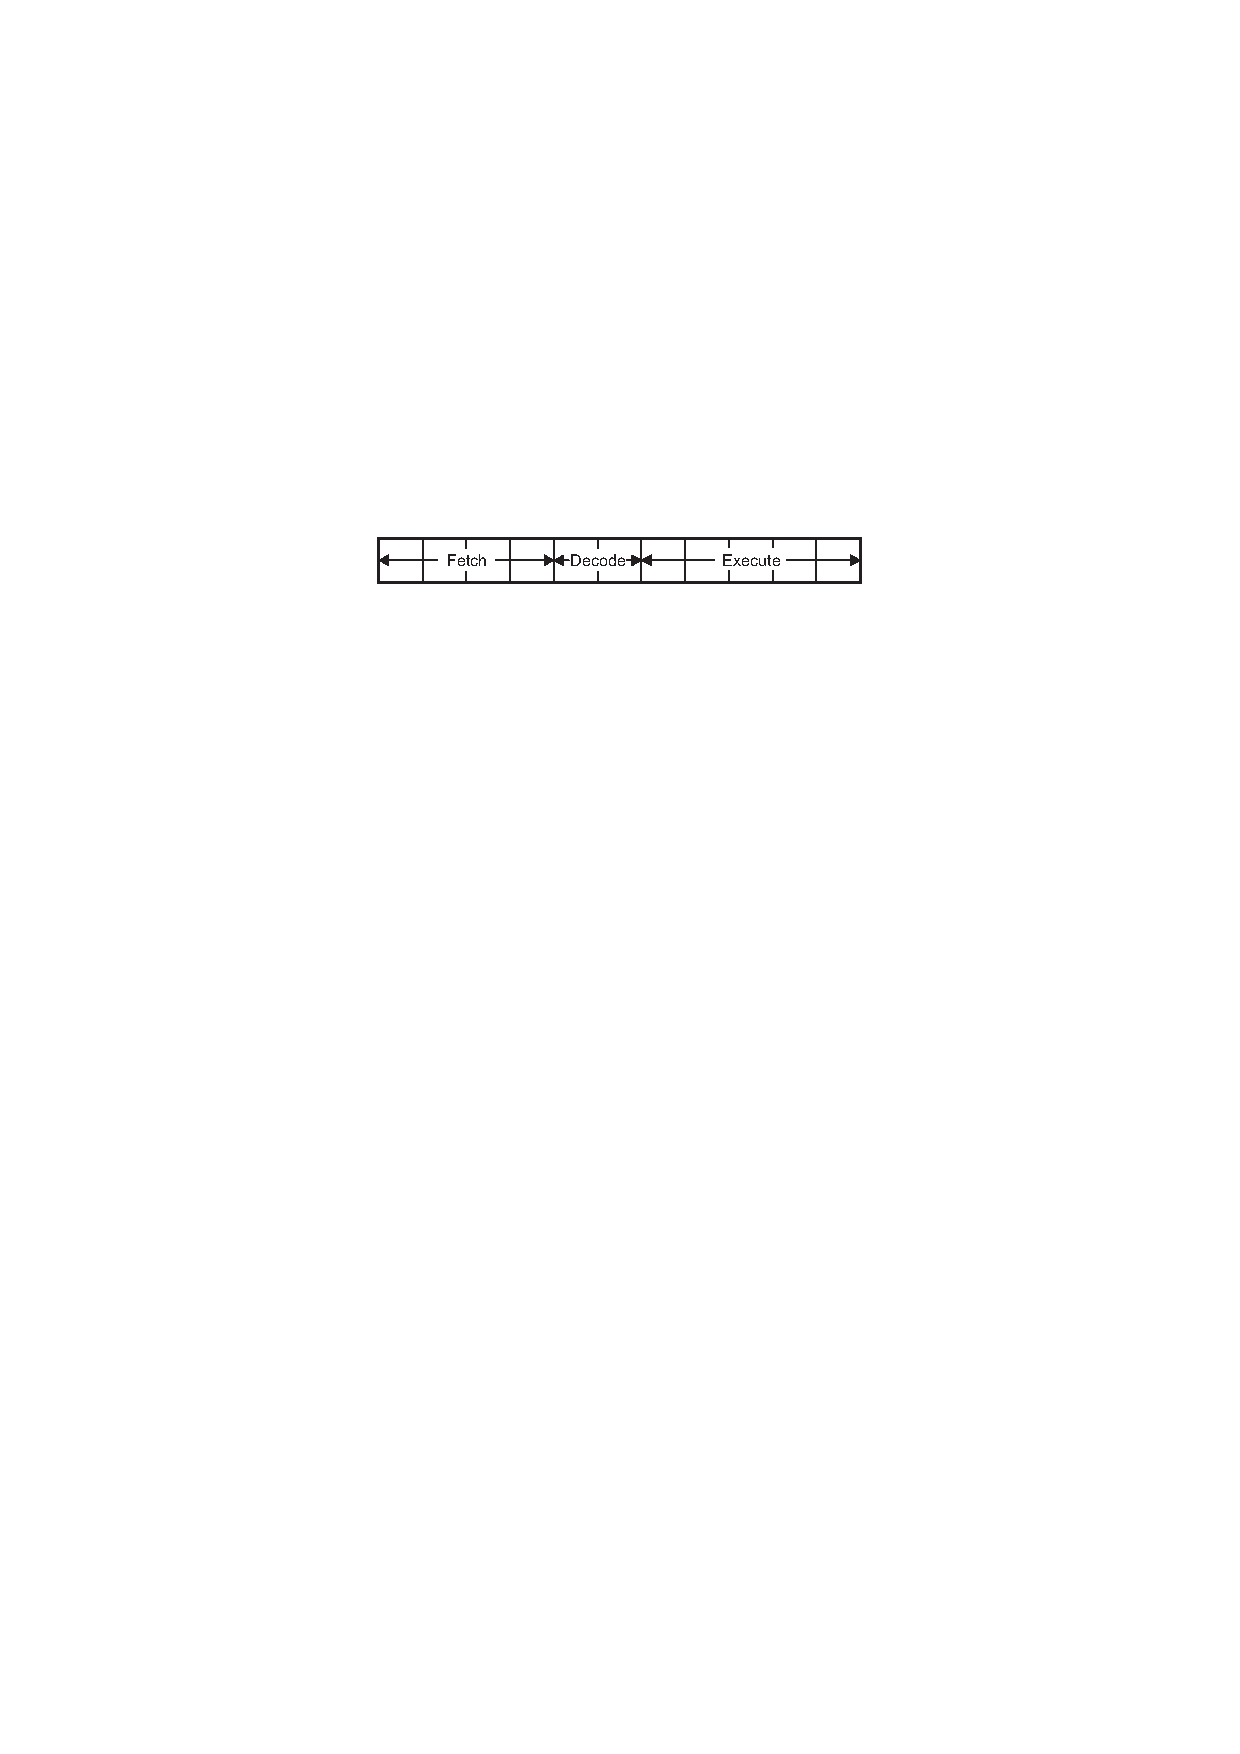
\includegraphics[width=1\textwidth]{../Pictures/dsppipe.pdf}
	\caption{Pipelinestufen und -phasen des C674x\cite{sprufe8b}}
	\label{fig:dsppipe}
\end{figure} 
% 
\subparagraph{Die Fetch-Phase}\label{subph:fetch}$\;$ \\\\
In der Fetch-Phase werden Befehle aus dem Instruktionscache geladen. Dieses ist wie bereits erw�hnt in vier Stufen unterteilt:

\begin{enumerate}
\item PG: Program address generate
\item PS: Program address send
\item PW: Program access ready wait
\item PR: Pregram fetch packet receive
\end{enumerate}

Zum Laden von Befehlen aus dem Instruktionscache wird ein sogenanntes Fetch Packet (FP) verwendet, welches aus acht Befehlen besteht. In einem Fetch Paket sind neben den acht Befehlen auch noch Informationen dar�ber enthalten, welche Befehle parallel ausgef�hrt werden k�nnen.

\subparagraph{Die Decode-Phase}$\;$ \\\\
Die Decode-Phase besteht aus zwei Stufen:
\begin{enumerate}
\item DP: Instruction dispatch
\item DC: Instruction decode
\end{enumerate}

In der DP-Phase werden die vorher geladenen Fetch Packets in sogenannte Execute Packets zerlegt. Hierbei stellt ein Execute Packet Befehle dar, die parallel auf den acht vorhandenen Ausf�hrungseinheiten bearbeitet werden k�nnen, daraus folgt, dass ein Execute Packet immer mindestens aus einem und maximal aus acht Befehlen bestehen kann. Au�erdem werden in dieser Phase den einzelnen Befehlen eines Execute Packets die Ausf�hrungseinheiten zugeordnet, die sie bearbeiten werden. Hierbei muss beachtet werden, dass Ausf�hrungseinheiten noch auf Grund von Latenzen belegt sein k�nnen (siehe \textbf{\ref{ph:reginst}}). Operationen die parallel bearbeitet werden sind im sp�teren Assembler-Code mit einem \glqq ||\grqq\  gekennzeichnet.\\
W�hrend der DC-Phase werden die Quell- und Zielregister und gegebenenfalls zugewiesene Crosspaths dekodiert, welche bei der sp�teren Ausf�hrung ben�tigt werden. 

\subparagraph{Die Execute-Phase}$\;$ \\\\
In der Execute-Stufe werden die vorher geladenen und decodierten Befehle auf den Hardwareeinheiten ausgef�hrt. Diese Stufe wird formell in zehn Stufen unterteilt, E1-E10, in denen je nach Befehl Lade- und/oder Schreiboperationen ausgef�hrt werden. Hierbei kann es allerdings passieren, dass bei manchen Befehlen eine bestimmte Zeit vergeht, bis das Ergebnis am Ausgang anliegt, diese Zeit wird als Delayslots bezeichnet und welche ab der Phase E1 gez�hlt werden (vgl. \textbf{Tabelle \ref{tab:c674x}}). Die maximale Anzahl an Delayslots im Instruktionssatz des C674x betr�gt 9.\\

\subparagraph*{Die Execute-Phase bei Double-Precision}$\;$ \\\\
Durch die Besonderheit von Double-Precision-Funktionen Operanden und Ergebnisse in zwei Schritten zu lesen, bzw. zu schreiben, ergeben sich M�glichkeiten diese beim Scheduling solcher Funktionen auszunutzen. Hierbei werden immer erst die LSBs gelesen, bzw. geschrieben und einen Takt sp�ter die MSBs.\\
Soll zum Beispiel erst eine Multiplikation (MPYSP2DP) und danach eine Addition (ADDDP) dieses Ergebnisses mit einem andern Wert geschehen, so kann die Addition bereits in dem Takt mit der Bearbeitung anfangen, in dem das LSB des Ergebnisses der Multiplikation geschrieben wurde.

\subsubsection{Code Parallelisierung durch Software Pipelined Loop (SPLOOP)}\label{ph:sploop}
Wenn Schleifen optimiert werden sollen gibt es neben Loop-Unrolling meistens keine andere M�glichkeit. Dieses Unrolling nutzt aber nicht effektiv alle acht Ausf�hrungseinheiten des DSPs aus.
Hier kommt die Software Piplined Loop ins spielt.\\ 
SPLOOP besteht zum einen Teil aus Hardware und zum anderen Teil aus Planungsarbeit, die w�hrend der Kompilierung vom Compiler aufgebracht wird.\\
Hierbei wird eine M�glichkeit geboten, Schleifen, welche im Programm vorkommen, in Form einer Pipeline abzuarbeiten. Hierf�r sind Hardwarekomponenten innerhalb des C674x vorhanden:

\begin{itemize}
\item Loop Buffer
\item Loop buffer count register (LBC)
\item Inner loop count register (ILC)
\item Reload inner loop count register (RILC)
\item Task state register (TSR)
\item Interrupt task state register (ITSR)
\item NMI/Exception task state register (NTSR)
\end{itemize}

Als erstes wird w�hrend der Kompilierung ein Ausf�hrungsplan aufgestellt, wodurch sequentiell kodierte Befehle aus verschiedenen Iterationsschritten parallel verarbeitet werden.\\
Hierf�r wird ein Iterationsschritt in sogenannte Stages unterteilt. Eine Stage bezeichnet hierbei einen Teil des sequentiell auszuf�hrenden Codes eines Interationsschritts, der sich dadurch auszeichnet, dass er eine vorgegebene Ausf�hrungszeit in Takten besitzt. Diese Ausf�hrungszeit wird als Iterationsintervall bezeichnet.\\
Wenn die Pipeline der SPLOOP vollst�ndig gef�llt ist, werden alle Stages parallel ausgef�hrt und jede Stage ist einem anderen Iterationsschritt zugeordnet. Dieses wird als Kernel bezeichnet. Die Phase vor dem Kernel wird als Prolog bezeichnet, die nach diesem als Epilog. \textbf{Abbildung \ref{fig:sploop}} soll dieses verdeutlichen.\\
%
\begin{figure}[htb]
	\centering
		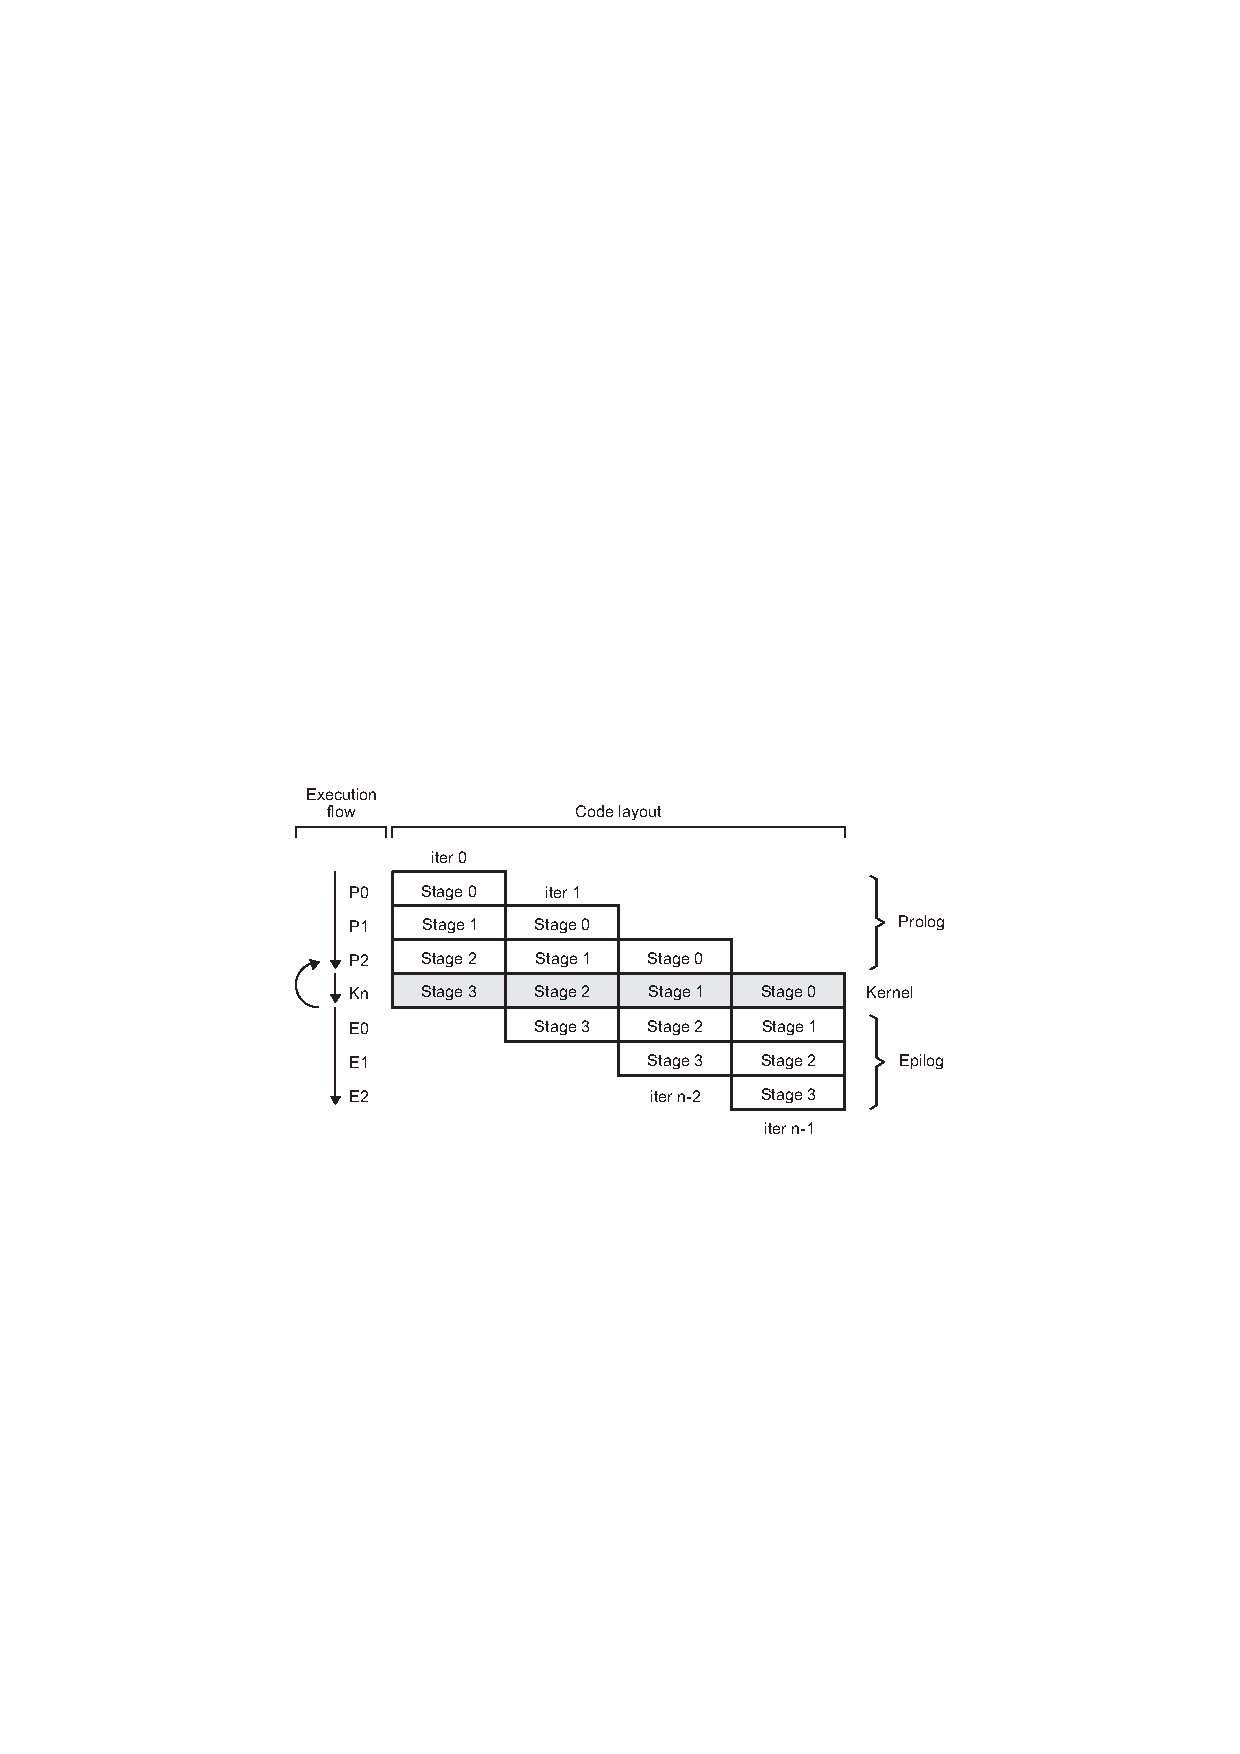
\includegraphics[width=1\textwidth]{../Pictures/sploop.pdf}
	\caption{Software Pipelined Execution Flow\cite{sprufe8b}}
	\label{fig:sploop}
\end{figure} 
% 
Um SPLOOP w�hrend der Ausf�hrung zu erm�glichen werden, SPLOOP-spezifische Befehle in den Assemblercode eingef�gt, die der zugrundeliegenden Hardware erm�glichen, Stages etc. zu erkennen. Diese Befehle lassen sich grob in drei Gruppen unterteilen:

\begin{itemize}
\item SPLOOP(D/W): Diese Befehlsgruppe l�sen den Loop Buffer Mechanismus aus
\item SPKERNEL(R): Diese Befehle markieren das Ende einer SPLOOP
\item SPMASK(R): Mit dieser Befehlsgruppe lassen sich einzelne Operationen auf Ausf�hrungseinheiten innerhalb eines Execute Packets sperren
\end{itemize}

\paragraph{Loop Buffer}$\;$ \\\\
Im Loop Buffer werden die f�r die Schleife ben�tigten Instruktionen, Informationen, ob diese momentan aktiv oder inaktiv sind und Informationen �ber ihre Abarbeitungsreihenfolge gespeichert. Diese Instruktionen werden in Form von Execute Packets gespeichert und es k�nnen bis zu 14 solcher Pakete hinterlegt werden.\\
Die Speicherung von Instruktionen im Loop Buffer bietet den Vorteil, dass sie nicht f�r jede Ausf�hrung neu die Fetch-Stufe durchlaufen m�ssen, sondern einfach aus dem Loop Buffer geladen werden k�nnen.\\
Aus diesem Buffer lie�t die Hardwareeinheit, der SPLOOP, die die parallele Abbarbeitung erm�glicht.

\paragraph{Loop buffer count register (LBC)}$\;$ \\\\
Das LBC fungiert als Inhaltsverzeichnis f�r den Loop Buffer und gibt an, welche Stages ausgef�hrt werden m�ssen. Das LBC wird in zwei F�llen auf null zur�ckgesetzt. Entweder wenn ein Befehl aus der SPLOOP(D/W)-Befehlsgruppe ausgef�hrt wird, oder wenn der Iterationsintervall-Wert erreicht ist, der beim letzten Befehl der eben genannten Gruppe mit �bergeben wurde. Sollte der zweite Fall eintreten, wird das ILC um 1 dekrementiert.\\
Es sind zwei LBCs vorhanden um eine Unterst�tzung f�r verschachtelte Schleifen zu gew�hrleisten.

\paragraph{Inner loop count register (ILC)}$\;$ \\\\
Im ILC ist die Gesamtzahl der Durchl�ufe hinterlegt, die f�r die Ausf�hrung der Schleife erforderlich sind. Erreicht das LBC den Iterationsintervall-Wert, wird das ILC dekrementiert, erreicht das ILC den Wert 0, endet die SPLOOP.

\paragraph{Reload inner loop count register (RILC)}$\;$ \\\\
Das RILC ist daf�r zust�ndig den ILC f�r die n�chste Ausf�hrung einer verschachtelten Schleife zur�ckzusetzen.

\paragraph{TSR, ITSR und NTSR}$\;$ \\

Diese drei Register sind f�r den Status der SPLOOP zust�ndig.\\
TSR zeigt an, ob eine SPLOOP momentan ausgef�hrt wird.\\
Sollte ein Interrupt kommen, wird der Inhalt des TSR in das ITSR kopiert.\\
Sollte ein Fehler oder ein nicht maskierbarer Interrupt auftreten, wird der Inhalt von TSR in NTSR kopiert.

\paragraph{Beispiel des Software-Pipelinings (SPLOOP)}\label{ph:bspsploop}$\;$ \\\\
Die Funktionsweise von SPLOOP soll nachfolgend am Beispiel der Schleife innerhalb der Berechnung des \textit{Spectral Centroids} erl�utert werden. \textbf{Listing \ref{code:scc}} zeigt den C-Code dieser Schleife und \textbf{Listing \ref{code:scasm}} den entsprechenden Assembler-Code.

\begin{lstlisting}[caption=C-Code der Schleife des Spectral Centroids, label=code:scc]
	for (k = 0; k < scsize; ++k) {
		weighted += A[k] * ((realv) k);
		total += A[k];
	}
\end{lstlisting}

\begin{lstlisting}[caption=Assembler-Code der Schleife des Spectral Centroids, label=code:scasm]
;** --------------------------------------------------------------------------*
$C$L1:    ; PIPED LOOP PROLOG

           SPLOOPD 4       ;12               ; (P) 
||         MV      .L1     A4,A6
||         MV      .S1X    B7,A8
||         MVC     .S2     B5,ILC

;** --------------------------------------------------------------------------*
$C$L2:    ; PIPED LOOP KERNEL

           INTSP   .L1     A8,A4             ; |2| (P) <0,0> 
||         LDW     .D1T1   *A6++,A5          ; |2| (P) <0,0> 

           NOP             2
           ADD     .S1     1,A8,A8           ; |1| (P) <0,3> Define a twin register
           NOP             1

           ADDSP   .L2X    A5,B4,B4          ; |3| (P) <0,5>  ^ 
||         MPYSP   .M1     A5,A4,A3          ; |2| (P) <0,5> 

           NOP             2
           NOP             1
	
           SPKERNEL 1,2
||         ADDSP   .L1     A3,A7,A7          ; |2| <0,9>  ^ 

;** --------------------------------------------------------------------------*
$C$L3:    ; PIPED LOOP EPILOG
;** --------------------------------------------------------------------------*
\end{lstlisting}
In diesem speziellen Beispiel ist der Epilog leer, dieses gilt aber nicht f�r die Allgemeinheit.\\
Wie durch den Befehl \textit{SPLOOPD 4} angegeben ist, betr�gt die L�nge eines Iterationsintervals vier Takte. Des weiteren sind sechs Stages vorhanden (innerhalb des Codes durch Leerzeilen getrennt), die jeweils vier Takte lang sind. Die einzige Ausnahme ist der Befehl \textit{LDW}, dieser wird in f�nf Takten ausgef�hrt, da allerdings nicht direkt nach dem 5. Takt aus A5 gelesen wird, stellt das kein Problem dar. Der Befehl \textit{SPKERNEL} markiert das Ende des Kernels, die Argumente dieses Befehls geben an, wie lange nach dem letzten Durchlauf gewartet werden muss, bis wieder Operationen ausgef�hrt werden k�nnen, in diesem Fall muss die Laufzeit einer Stage und 2 Takte gewartet werden, also insgesamt 6 Takte.\\
Die Konstante \textit{scsize} steht f�r die halbe Breite eines betrachteten Fensters. Die Berechnung der Gesammtlaufzeit einer Schleife mit SPLOOP wird nach \textbf{Formel \ref{eqn:sploop}} berechnet. Im Fall des \textit{Spectral Centroids} mit einer Fensterbreite von 512, betr�gt die Gesamtlaufzeit in Takten 976.

\begin{equation}\label{eqn:sploop}
Zeit~=~ \left[\overbrace{\#Stages}^{Einschwung}+\overbrace{\left(\frac{\#Durchl"aufe - 2 \cdot \#Stages}{\#Stages}\right)}^{Eingeschwungen}+\overbrace{\#Stages}^{Ausschwung}\right] \cdot Iterationsinterval
\end{equation}

\subsubsection{Compileroptimierungsstufen}
In diesem Kapitel sollen die Optimierungsstufen des DSP-Compilers aus dem bereits vorgestellten C6EZRun-Framework (siehe \textbf{Kapitel \ref{sec:c6run}}) erl�utert werden.\\
Da dieser Compiler auf dem C6000-DSP-Compiler aufsetzt, k�nnen auch die Compileroptimierungen des C6000-Compilers verwendet werden, Diese Optimierungsstufen optimieren auf Geschwindigkeit.\\
Dieser besitzt neben den g�ngigen Optimierungsstufe O0-O3, auch die M�glichkeit eine softwarebasierte Pipelinestruktur zu verwenden, die sich Software Pipelined Loop oder kurz SPLOOP nennt.

\paragraph{Optimierungsstufe \-O0}$\;$ \\\\
In der niedrigsten Optimierungsstufe, welche entweder durch das Compilerflag \textit{\-opt\_level=0} oder \textit{\-O0} aufgerufen wird, werden nur einfache Optimierungen des Codes durchgef�hrt:

\begin{itemize}
\item Kontrollfluss-Graph-Vereinfachung
\item Allokierung von Variablen auf Register
\item Loop Rotation 
\item Eliminierung von unbenutztem Code
\item Vereinfachung von Ausdr�cken und Statements
\item Unterst�tzung von Inline-Funktionen 
\end{itemize}

\paragraph{Optimierungsstufe \-O1}$\;$ \\

Die n�chst h�here Optimierungsstufe wird mit dem Compilerflag  \textit{\-opt\_level=1} oder \textit{\-O1} aufgerufen. Diese Stufe schlie�t alle Optimierungen der Stufe 0 ein und erweitert diese um:

\begin{itemize}
\item Durchf�hrung von lokalen Kopier- und Konstantenpropagation
\item Entfernung von �berfl�ssigen Anweisungen
\item Lokale Eliminierung von mehrfach verwendeten Ausdr�cken
\end{itemize}

\paragraph{Optimierungsstufe \-O2}$\;$ \\

Die Optimierungsstufe 2 wird mit dem Compilerflag \textit{\-opt\_level=2} oder \textit{\-O3} aufgerufen und erweitert die Optimierungsstufe 1 um:

\begin{itemize}
\item Optimierung f�r Verwendung der Software Pipelined Loop (\textbf{\ref{ph:sploop}})
\item Schleifenoptimierung
\item Eliminierung von globalen verbreiteten Ausdr�cken
\item Eliminierung von globalen �berfl�ssigen Ausdr�cken
\item Konvertierung von Arrayreferenzen in Schleifen zu Pointerarithmetik
\item Loop Unrolling
\end{itemize}

\paragraph{Optimierungsstufe \-O3}\label{ph:o3}$\;$ \\

Die letzte Optimierungsstufe wird mit \textit{\-opt\_level=3} oder \textit{\-O3} aufgerufen. Auch diese schlie�t alle Optimierungen der vorherigen Stufen ein, au�erdem kommen folgende dazu:

\begin{itemize}
\item Entfernung von unverwendeten Funktionen
\item Vereinfachung von Funktionen, deren R�ckgabewert nie verwendet wird
\item Inline Calls zu kleinen Funktionen
\item Neusortierung von Funktionsdeklarationen
\item Propagierung von Argumenten in den Funktionsk�rper, wenn alle Aufrufe den selben Wert an der selben Position besitzen
\item Identifizierung von File-Level Charakteristiken von Variablen
\end{itemize}

\paragraph{Beispiel der Compileroptimierung}\label{ph:bspcomp}$\;$ \\\\
Anhand des \textit{Root Mean Square} soll hier die Optimierung O3 des C6EZRun-Compilers verdeutlicht werden. Hierf�r soll neben den Optimierungen aus \textbf{Kapitel \ref{ph:o3}} auch die Pipeline aus \textbf{Kapitel \ref{ph:dsppipe}} gezeigt werden.\\
\textbf{Listing \ref{code:rmsc}} zeigt den C-Code des \textit{Root Mean Square} und \textbf{Listing \ref{code:rmsasm}} den daraus Kompilierten Assembler-Code.

\begin{lstlisting}[caption=C-Code des Root Mean Square, label=code:rmsc]
	for (n = 0; n < rmsinfo.N; ++n) {
		mean += ((realv) signal[n] / (realv) rmsinfo.N)
		* (realv) signal[n];

	}

	rms[run] = sqrt(mean);
\end{lstlisting}

\begin{lstlisting}[caption=Assembler-Code des Root Mean Square, label=code:rmsasm]
           CMPGT   .L1     A3,0,A0           ; |1| 
||         INTSP   .L2X    A3,B10
||         MV      .S1     A3,A10            ; |2| 
   [!A0]   BNOP    .S1     $C$L2,5           ; |1| 
|| [ A0]   LDW     .D1T1   *A13++,A15        ; |2| 
	   CALL    .S1     __c6xabi_divf     ; |2| 
           MV      .L2     B10,B4            ; |2| 
           MV      .L1     A15,A4            ; |2| 
           NOP             2
           MPYSP   .M1     A15,A4,A3         ; |2| 
||         SUB     .L1     A10,1,A0          ; |1| 
   [ A0]   LDW     .D1T1   *A13++,A15        ; |2| 
|| [ A0]   B       .S1     $C$L1             ; |1| 
   [ A0]   CALL    .S1     __c6xabi_divf     ; |2| 
   [ A0]   MV      .L2     B10,B4            ; |2| 
           ADDSP   .L1     A3,A14,A14        ; |1| 
           SUB     .L1     A10,1,A10         ; |1| 
   [ A0]   MV      .L1     A15,A4            ; |2|  
	   CALLP   .S2     sqrt,B3
||         SPDP    .S1     A14,A5:A4         ; |7|   
           DPSP    .L1     A5:A4,A3          ; |7| 
           NOP             1
           STW     .D1T1   A3,*+A12[A11]     ; |7| 
\end{lstlisting}

Zur Erl�uterung der Leseweise des Assembler-Codes, sei gesagt, dass ein || am Anfang einer Zeile bedeutet, dass der folgende Befehl parallel zum Befehl der vorherigen Zeile ausgef�hrt wird. Die vierte Spalte gibt den Datenpfad und die entsprechende Ausf�hrungseinheit an, so wird zum Beispiel das \textit{Zero} aus Zeile 11 im Datenpfad 1 auf der L-Einheit ausgef�hrt, |n| steht f�r die Entsprechende Zeile aus dem C-Code in \textbf{Listing \ref{code:rmsc}} (Zeile 2 und 3 werden als Zeile 2 gewertet).\\
Wie in \textbf{Kapitel \ref{subph:fetch}} bereits erw�hnt, werden immer acht Befehle zu einem Fetch Packet zusammen gefasst, so das die 23 Befehle zu drei solchen Paketen zusammen gefasst werden k�nnen (vgl. \textbf{Tabelle \ref{tab:fetch}}).

\begin{table}[ht]
\centering
\begin{tabular}{|c|c|c|c|c|c|c|c|c|}
\hline
FP Nummer & Slot 1 & Slot 2 & Slot 3 & Slot 4 & Slot 5 & Slot 6 & Slot 7 & Slot 8\\
\hline\hline
1 & cmpgt & intsp & mv & bnop & ldw & call & mv & mv\\
2 & nop & mpysp & sub & ldw & b &call& mv &addsp\\
3 & sub & mv & callp & spdp & dpsp & nop &stw &nop\\
\hline
\end{tabular}
\caption{Fetch Pakets des Root Mean Square Assembler-Codes}
\label{tab:fetch}
\end{table}

W�hrend der Decode-Stufe werden danach Zuordnungen zu Execute Pakets durchgef�hrt, wo zum Beispiel f�r Fetch Paket 1 festgestellt wurde, dass es in f�nf solcher Execute Pakets gesplittet werden kann. Diese Execute Pakets wurden danach den Ausf�hrungseinheiten zugeordnet und in der Execute-Stufe ausgef�hrt.\\
An Optimierungen lassen sich hierzum Beispiel nennen: 
\begin{itemize}
\item Die Inline Calls zu \textit{sqrt} und \textit{\_\_c6xabi\_dif}
\item Die Konvertierung von Array-Aufrufen in Pointerarithmetiken, z.B. in Zeile 5.
\item Die Propagation von Konstanten in Register, z.B. rmsinfo.N in A0
\end{itemize} 

\subsubsection{Optimierte Bibliotheken f�r den C674x}
Texas Instruments bietet zu seinen DSPs der C6000-Reihe auch noch eine Reihe Bibliotheken an, diese enthalten Algorithmen die speziell f�r DSPs dieser Baureihe optimiert wurden. Einige dieser optimierten Bibliotheken sind im Umfang des EZSDK (siehe \textbf{Kapitel \ref{sec:ezsdk}})enthalten. Im Folgenden werden zwei dieser Bibliotheken n�her vorgestellt, zum einen die DSPLIB mit Algorithmen aus der Signalverarbeitung und zum anderen die MATHLIB mit optimierten mathematischen Funktionen.

\paragraph{DSPLIB}$\;$ \\\\
Wie schon erw�hnt ist die DSPLIB-Bibliothek eine Zusammenfassung von Algorithmen aus der Signalverarbeitung, die f�r den Gebrauch auf DSPs der C6000-Reihe optimiert wurde und direkt von Texas Instruments stammt. Diese liegen innerhalb dieser Bibliothek sowohl als C- als auch als Assembler-Code vor.

\paragraph{MATHLIB}$\;$ \\

Die MATHLIB-Bibliothek ist ebenfalls f�r die Verwendung auf DSPs der C6000-Reihe optimiert. Auch diese Bibliothek stammt von Texas Instruments. F�r diese Bibliothek liegen der Quellcode ebenfalls sowohl als C- als auch als Assembler-Code vor.\\
Die mathematischen Funktionen sind sowohl f�r Double-Precision als auch f�r Single-Precision vorhanden und bieten neben der Option einzelne Aufrufe auszuf�hren, auch die M�glichkeit Operationen auf Arrays auszuf�hren. Werden diesen Arrayoperationen zum Beispiel die Array a und b �bergeben, wird immer das n-te Element von a mit dem n-ten Element von b verrechnet.

\section{Linux EZ Software Development Kit (EZSDK)}\label{sec:ezsdk}
Das Linux EZ Software Development Kit (EZSDK) ist eine von Texas Instruments zum EVM816x-Board mitgelieferte Sammlung von wichtigen und n�tzlichen Tools. Das EZSDK (gesprochen: \textit{EasySDK}) l�sst sich grob in vier Softwaregruppen unterteilen:

\begin{itemize}
\item Board Support
\begin{itemize}
\item Kernel f�r embedded Linux Version 2.6.37
\item U-Boot (Bootloader)
\item Sammlung von Tools auf System-on-Chip-Ebene
\end{itemize}
\item Component Sources
\begin{itemize}
\item Optimierte Bibliotheken f�r den DSP
\item Kommunikationsframeworks zwischen ARM und DSP
\item DSP-Betriebssystem
\item weitere Tools
\end{itemize}
\item DSP Development Kit (DSP-Toolchain)
\item Linux Development Kit (Linux-Toolchain)
\end{itemize}

F�r diese Arbeit wurde die EZSDK-Version 5.02 verwendet.

\section{C6EZRun}\label{sec:c6run}

C6EZRun ist ein Framework, welches f�r die Kommunikation zwischen ARM und DSP entwickelt wurde. Dieses Framework nimmt dem Programmierer wesentliche Aspekte der Kommunikation zwischen diesen beiden Prozessoren ab, zum Beispiel Kommunikationswege, Latenzzeiten, Speicherverwaltung, Pointerkonvertierungen, etc.\\
Hierbei sind zwei unterschiedliche M�glichkeiten zur Kommunikation zwischen ARM und DSP vorhanden:

\begin{itemize}
\item C6Runlib
\item C6Runapp
\end{itemize}

C6runlib bietet die M�glichkeit Teile des Programmcodes auf den DSP auszulagern. Hierbei werden die entsprechenden Programmteile in C-Code geschrieben und mit dem C6Runlib-Compiler zu einer Bibliothek compiliert. Diese Bibliothek kann anschlie�end in das bestehende Projekt eingef�gt und die in ihr enthaltenen Funktionen so aufgerufen werden, als wenn sie auf dem ARM laufen w�rden.\\
C6Runapp hingegen bietet die M�glichkeit ein komplettes Programm auf dem DSP auszuf�hren, dieses aber �ber die Konsole des ARM aufzurufen. Hierf�r wird der Programm-Code ebenfalls in C-Code beschrieben und mit dem C6Runapp-Compiler kompiliert.\\
Die in dieser Arbeit verwendete Version von C6EZRun ist 0.98.


%bibtex Referenzen in bib datei
\bibliography{references/references}
\bibliographystyle{Macros/unsrtdin}
%\bibliographystyle{unsrt}
%Literaturverzeichnis ins Inhaltsverzeichnis
\addcontentsline{toc}{chapter}{Literaturverzeichnis}

\appendix %%Anhang
\renewcommand{\chaptermark}[1]{\markright{Appendix \thechapter\ \it #1}}
\renewcommand{\sectionmark}[1]{\markright{Appendix \thechapter\ \it #1}}
\renewcommand{\appendixname}{Anhang}
\renewcommand{\tablename}{Table}
\renewcommand{\figurename}{Figure}

\input{Anhang/Anhang}
\newpage
\thispagestyle{empty}
\mbox{}

\end{document}
